% ---- paper/parts/S0_supplement_front.tex ----
%% ---------------------------------------------------------------------
%%  SUPPLEMENTARY MATERIAL for
%%  "Specification Surfaces for Incremental Predictive Performance"
%%
%%  Round twenty-one.  The developmental review's twelfth comment is that the
%%  manuscript is ninety-seven pages, roughly thirty of them about the
%%  project's own history of errors, and that no reviewer finishes it.  This
%%  document is where that material lives.  The main text is self-contained;
%%  nothing here is needed to follow it, and every number here is the same
%%  macro the main text uses, generated by scripts/make_numbers.py from
%%  results/*.csv.
%%
%%  Cross-references INTO the main text resolve through the `xr' package, so
%%  a reference here to Section 4 or Table 6 is a reference to that document's
%%  own numbering.  Sections, tables and figures in THIS document carry an S.
%% ---------------------------------------------------------------------
\documentclass[preprint,12pt]{elsarticle}

\usepackage{lmodern}
\usepackage{amsmath}
\usepackage{amssymb}
\usepackage{amsthm}
\usepackage{graphicx}
\usepackage{booktabs}
\usepackage{array}
\usepackage[hyphens]{url}
\urlstyle{rm}
\usepackage[protrusion=true,expansion=false]{microtype}
\usepackage{xr}

\makeatletter
\DeclareRobustCommand\texttt[1]{%
  {\ttfamily\hyphenchar\font=`\-\relax #1}}
\makeatother
\setlength{\emergencystretch}{3em}

\usepackage[section]{placeins}
\renewcommand{\topfraction}{0.9}
\renewcommand{\bottomfraction}{0.8}
\renewcommand{\textfraction}{0.07}
\renewcommand{\floatpagefraction}{0.7}
\setcounter{topnumber}{3}
\setcounter{totalnumber}{5}

%% GENERATED by scripts/make_numbers.py -- do not edit.
%% Every numeric literal in the manuscript is one of these.
\newcommand{\Dabs}{+0.0899}
\newcommand{\DabsHi}{+0.1256}
\newcommand{\DabsLo}{+0.0634}
\newcommand{\Rref}{0.350}
\newcommand{\RrefKind}{bounded}
\newcommand{\VCorruptDelta}{-0.0357}
\newcommand{\VDuplicateDelta}{-0.0003}
\newcommand{\VPopCommon}{+0.1055}
\newcommand{\VPopRare}{+0.1039}
\newcommand{\VStaleDelta}{+0.0000}
\newcommand{\VTone}{+0.1835}
\newcommand{\VToneLo}{+0.1650}
\newcommand{\VTonehi}{+0.1909}
\newcommand{\VTtwoGroup}{+0.1033}
\newcommand{\VTtwoGroupHi}{+0.1106}
\newcommand{\VTtwoGroupLo}{+0.0762}
\newcommand{\VTtwoKnow}{-0.0032}
\newcommand{\VTtwoKnowHi}{+0.0013}
\newcommand{\VTtwoKnowLo}{-0.0079}
\newcommand{\agreeTolerance}{$1.1 \times 10^{-16}$}
\newcommand{\auditBJustifiedPct}{18\%}
\newcommand{\auditBStatedPct}{85\%}
\newcommand{\auditBoundHi}{48\%}
\newcommand{\auditBoundLo}{9\%}
\newcommand{\auditHalfWidthPct}{18 percentage points}
\newcommand{\auditKappa}{0.20}
\newcommand{\auditMJustifiedPct}{5\%}
\newcommand{\auditMaxWeight}{1.00}
\newcommand{\auditPrec}{0.481}
\newcommand{\auditPrecReg}{0.301}
\newcommand{\auditRangeBaselinePct}{34\%}
\newcommand{\auditRangeMetricPct}{15\%}
\newcommand{\auditRangePopulationPct}{0\%}
\newcommand{\auditRangeThresholdPct}{5\%}
\newcommand{\auditSens}{0.474}
\newcommand{\auditSensHi}{0.602}
\newcommand{\auditSensLo}{0.347}
\newcommand{\auditSensReg}{0.569}
\newcommand{\auditSpec}{0.911}
\newcommand{\auditSpecReg}{0.769}
\newcommand{\auditThetaStatedPct}{27\%}
\newcommand{\biasNoisyBefore}{-0.0353}
\newcommand{\biasOracleMax}{0.0405}
\newcommand{\cardF}{3{,}019}
\newcommand{\casePrevalence}{0.372}
\newcommand{\corruptLevel}{15\%}
\newcommand{\coverageNaiveMedian}{90.5\%}
\newcommand{\coverageNaiveMin}{5.5\%}
\newcommand{\coverageNestedBasicMedian}{92.0\%}
\newcommand{\coverageNestedBasicMin}{7.0\%}
\newcommand{\coverageNestedBcMedian}{91.5\%}
\newcommand{\coverageNestedMedian}{94.2\%}
\newcommand{\coverageNestedMin}{3.5\%}
\newcommand{\coverageNoisyAfter}{7.0\%}
\newcommand{\coverageNoisyBefore}{7.0\%}
\newcommand{\crossTargetAgreement}{45\%}
\newcommand{\doiBPICfourteen}{\url{https://doi.org/10.4121/uuid:c3e5d162-0cfd-4bb0-bd82-af5268819c35}}
\newcommand{\doiBPICthirteen}{\url{https://doi.org/10.4121/uuid:500573e6-accc-4b0c-9576-aa5468b10cee}}
\newcommand{\exCells}{480}
\newcommand{\exMisreportPct}{24.9\%}
\newcommand{\exRmax}{0.947}
\newcommand{\exRmin}{0.200}
\newcommand{\exRows}{30{,}162}
\newcommand{\exSbaselinePct}{25.9\%}
\newcommand{\exSmetricPct}{25.9\%}
\newcommand{\exSpopulationPct}{7.2\%}
\newcommand{\exampleLines}{121}
\newcommand{\flipLearnerPct}{31.3\%}
\newcommand{\flipMetricPct}{19.7\%}
\newcommand{\flipQualityPct}{20.4\%}
\newcommand{\flipRungPct}{22.2\%}
\newcommand{\flipSplitPct}{33.5\%}
\newcommand{\fvVersion}{0.2.0}
\newcommand{\gridHi}{0.80}
\newcommand{\gridLo}{0.05}
\newcommand{\kmBaseAuc}{0.648}
\newcommand{\kmOrphanPopulated}{100\%}
\newcommand{\lambdaHalf}{0.64}
\newcommand{\lambdaHalfPct}{64\%}
\newcommand{\limitNoisyAfter}{+0.1135}
\newcommand{\limitNoisyBefore}{+0.1135}
\newcommand{\maxCardBZero}{200}
\newcommand{\maxTMedian}{4.03}
\newcommand{\maxTMedianRatio}{2.06}
\newcommand{\meanNoisyEstimate}{+0.0781}
\newcommand{\minCardF}{50}
\newcommand{\minGPresent}{50\%}
\newcommand{\minPerStratum}{25}
\newcommand{\minReuseF}{two}
\newcommand{\minTrainCoverage}{50\%}
\newcommand{\misreportMaxPct}{57.7\%}
\newcommand{\misreportMedianPct}{35.3\%}
\newcommand{\misreportMinPct}{5.6\%}
\newcommand{\nAgreeDisagree}{0}
\newcommand{\nAgreeQuantities}{266}
\newcommand{\nAuditApplicable}{3}
\newcommand{\nAuditEffective}{29.6}
\newcommand{\nAuditEligible}{54.9}
\newcommand{\nAuditFrame}{600}
\newcommand{\nAuditFullText}{369}
\newcommand{\nAuditNoFullText}{231}
\newcommand{\nAuditOutSampled}{120}
\newcommand{\nAuditRequired}{196}
\newcommand{\nAuditSampled}{600}
\newcommand{\nAuditScreenedIn}{54}
\newcommand{\nAuditScreenedOut}{315}
\newcommand{\nAuditStrata}{77}
\newcommand{\nAuditTarget}{2{,}400}
\newcommand{\nAxes}{nine}
\newcommand{\nBandResolvedRaw}{2{,}046}
\newcommand{\nBandResolvedRecentred}{2{,}163}
\newcommand{\nCaseTest}{13{,}637}
\newcommand{\nCaseTrain}{31{,}818}
\newcommand{\nClosedBefore}{5}
\newcommand{\nCohort}{45{,}455}
\newcommand{\nCohortCorpus}{46{,}606}
\newcommand{\nCondBeneficial}{11}
\newcommand{\nCondHarmful}{1}
\newcommand{\nConditions}{8}
\newcommand{\nConfirmReject}{5}
\newcommand{\nCorpusLogs}{21}
\newcommand{\nDomains}{6}
\newcommand{\nDrawRows}{1{,}791{,}720}
\newcommand{\nFieller}{10{,}584}
\newcommand{\nFiellerUnbounded}{5{,}282}
\newcommand{\nFolds}{five}
\newcommand{\nGrid}{31}
\newcommand{\nHarmfulPointwise}{0}
\newcommand{\nHarmfulSimultaneous}{0}
\newcommand{\nLearners}{4}
\newcommand{\nLogs}{13}
\newcommand{\nLogsBothTargets}{6}
\newcommand{\nMeanOptimal}{19}
\newcommand{\nMetrics}{36}
\newcommand{\nMisreportOverQuarter}{13}
\newcommand{\nMisreportOverTen}{18}
\newcommand{\nOneNumberOptimal}{9}
\newcommand{\nOrphans}{94{,}250}
\newcommand{\nPairs}{19}
\newcommand{\nPairsBanded}{19}
\newcommand{\nPenaltyDecades}{five}
\newcommand{\nPropN}{1{,}800}
\newcommand{\nPropP}{200}
\newcommand{\nQuality}{10}
\newcommand{\nResultEstates}{18}
\newcommand{\nResultPairs}{12}
\newcommand{\nScaleReps}{\textbf{??}}
\newcommand{\nSeeds}{three}
\newcommand{\nSignChanging}{4}
\newcommand{\nSignVaries}{18}
\newcommand{\nSimReps}{200}
\newcommand{\nSimSparse}{200}
\newcommand{\nSizeGrid}{six}
\newcommand{\nSplits}{6}
\newcommand{\nSurfaceRows}{262{,}656}
\newcommand{\nTests}{108}
\newcommand{\nTrainOnly}{122}
\newcommand{\nTrainOnlyPassed}{122}
\newcommand{\nUniformlyBeneficial}{1}
\newcommand{\nUnresolvedPairs}{2}
\newcommand{\nWorkedBefore}{41{,}413}
\newcommand{\nWorlds}{six}
\newcommand{\noisyGapLarge}{\textbf{??}}
\newcommand{\noisyGapLoose}{\textbf{??}}
\newcommand{\noisyGapSmall}{\textbf{??}}
\newcommand{\noisyGapTight}{\textbf{??}}
\newcommand{\pThreeRawA}{0.421}
\newcommand{\pThreeRawB}{0.284}
\newcommand{\pThreeSqrtA}{0.232}
\newcommand{\pThreeSqrtB}{0.390}
\newcommand{\prevHi}{0.95}
\newcommand{\prevLo}{0.05}
\newcommand{\propOneApGap}{0.988}
\newcommand{\propOneAucGap}{exactly zero}
\newcommand{\propOneSweepAp}{0.998}
\newcommand{\propOneSweepAuc}{$4.4 \times 10^{-15}$}
\newcommand{\propTwoCancelShift}{machine precision}
\newcommand{\propTwoNonRankShift}{11.696}
\newcommand{\propTwoRankShift}{exactly zero}
\newcommand{\qClean}{+0.1673}
\newcommand{\qCommonHalf}{+0.1055}
\newcommand{\qCorruptThirty}{-0.0699}
\newcommand{\qDuplicateAll}{-0.0038}
\newcommand{\qLagHalfDelta}{-0.0031}
\newcommand{\qLagHalfPopulated}{94.1\%}
\newcommand{\qRandomHalf}{+0.0951}
\newcommand{\qRareHalf}{+0.1039}
\newcommand{\qStaleDelta}{+0.0000}
\newcommand{\qStaleKeepsDelta}{+0.0000}
\newcommand{\ratioBase}{2.3}
\newcommand{\ratioCheap}{9.0}
\newcommand{\ratioDear}{0.7}
\newcommand{\regretMajority}{0.0297}
\newcommand{\regretMajorityAdj}{0.0197}
\newcommand{\regretMajorityGainAdjPct}{18.3\%}
\newcommand{\regretMajorityGainPct}{21.9\%}
\newcommand{\regretMeanRule}{0.0242}
\newcommand{\regretOneNumber}{0.0380}
\newcommand{\regretOneNumberAdj}{0.0241}
\newcommand{\regretOneNumberExcessPct}{57.2\%}
\newcommand{\regretOracle}{0.0242}
\newcommand{\regretUniformRule}{0.0489}
\newcommand{\releaseTag}{v19.0}
\newcommand{\resultWitnessMax}{5}
\newcommand{\resultWitnessMin}{0}
\newcommand{\rhoMedian}{0.200}
\newcommand{\shiftMedian}{-0.0001}
\newcommand{\shiftNegativePct}{56\%}
\newcommand{\simNoiseRate}{20\%}
\newcommand{\simPrevalence}{0.02}
\newcommand{\sizeHi}{\textbf{??}}
\newcommand{\sizeLo}{\textbf{??}}
\newcommand{\sobolInteractionPct}{30.0\%}
\newcommand{\sobolLearnerPct}{2.6\%}
\newcommand{\sobolMaxAxis}{the metric}
\newcommand{\sobolMaxPct}{10.1\%}
\newcommand{\sobolMetricPct}{10.1\%}
\newcommand{\sobolQualityPct}{2.7\%}
\newcommand{\sobolRungPct}{1.9\%}
\newcommand{\sobolSplitPct}{9.4\%}
\newcommand{\sobolTargetPct}{2.1\%}
\newcommand{\sobolTopAxis}{the split}
\newcommand{\sobolTopPair}{BPIC19/duration}
\newcommand{\sobolTopPct}{50.7\%}
\newcommand{\sparseGapLarge}{\textbf{??}}
\newcommand{\sparseGapSmall}{\textbf{??}}
\newcommand{\spreadHeadline}{0.091 AUC at the median pair and 0.298 at the widest}
\newcommand{\spreadMax}{0.298}
\newcommand{\spreadMedian}{0.091}
\newcommand{\targetAgreement}{51\%}
\newcommand{\targetAgreementHi}{66\%}
\newcommand{\targetAgreementLo}{43\%}
\newcommand{\thetaBase}{0.30}
\newcommand{\thetaCheap}{0.10}
\newcommand{\thetaDear}{0.60}
\newcommand{\unseenMax}{87\%}
\newcommand{\unseenMin}{0\%}
\newcommand{\widthNoisyBefore}{0.0367}
\newcommand{\zenodoDOI}{the archived release cited in the data-availability statement (DOI reserved, inserted at proof)}


%%  The main text's labels, so that a reference from here to a section or a
%%  table of the article resolves to the article's own number.
\externaldocument{specification_surfaces}

\newtheorem{proposition}{Proposition}
\newtheorem{lemma}{Lemma}
\newtheorem{corollary}{Corollary}
\newtheorem{definition}{Definition}
\newtheorem{remark}{Remark}
\theoremstyle{definition}
\newtheorem{assumption}{Assumption}

%%  S-numbering, so a reader holding both documents can never confuse
%%  Table 6 with Table S6.
%%  The contents list boxes a section number in a width sized for `11.'; an
%%  `S11.3' overruns it and LaTeX reports ninety overfull boxes for the list
%%  alone.  Widening the boxes is the fix; the alternative, dropping the
%%  contents list from a forty-page supplement, costs the reader more.
\usepackage{tocloft}
\setlength{\cftsecnumwidth}{3.4em}
\setlength{\cftsubsecnumwidth}{4.2em}
\setlength{\cftsubsecindent}{3.4em}

\renewcommand{\thesection}{S\arabic{section}}
\renewcommand{\thetable}{S\arabic{table}}
\renewcommand{\thefigure}{S\arabic{figure}}
\renewcommand{\theproposition}{S\arabic{proposition}}
\renewcommand{\thelemma}{S\arabic{lemma}}
\renewcommand{\thecorollary}{S\arabic{corollary}}
\renewcommand{\theassumption}{S\arabic{assumption}}
\renewcommand{\theremark}{S\arabic{remark}}

\journal{Information Systems}

\begin{document}

\begin{frontmatter}

\title{Supplementary material for\\
\emph{Specification Surfaces for Incremental Predictive Performance:
Estimation, Uncertainty, and Multi-Log Evaluation}}

\author[ind]{Sudhir Dixit}
\ead{sudhir.dixit1@gmail.com}
\address[ind]{Independent Researcher}

\begin{abstract}
This document holds the protocol and its amendments, the proofs, the
constructions of the reporting objects, the correction register, the
per-layer and per-fold results, the literature pilot, the diagnosis of the
one simulated world where the bootstrap misbehaves, the worked example, the
verification harness, the derivation of the coverage calibration, three
results the article summarises in a paragraph each --- the family-by-encoding
crossing, the decision-rule comparison, and the calibration, unseen-category
and rolling-origin diagnostics --- and the tables the article does not print.
The article is self-contained without it. Every number in both documents is
generated from the same result files by the same script, so a quantity cannot
differ between them.
\end{abstract}

\end{frontmatter}

\tableofcontents
\clearpage
% ---- paper/parts/S9_supplement_back.tex ----
\section{Protocol, and the amendments to it}
\label{app:protocol}

The corpus protocol is \texttt{PROTOCOL.md} and the practice pilot's is
\texttt{AUDIT-PROTOCOL-2.md}; both are in the archive and both were committed
before the first result they govern existed. This appendix lists what changed
afterwards.

\paragraph{Why amendments are reported rather than folded in}
A pre-registration that is quietly edited is worse than none, because it
claims a discipline it does not have. Each amendment below names its date, the
defect that forced it, and the result it moved.

\begin{description}
\item[Amendment 1 --- a register's values must recur across time.]
Registered rule 3.3 admits any attribute reused across two cases on average.
On BPI Challenge 2019 that admits the purchasing-document number, which is a
document identifier and not a maintained entity: almost none of its values
recur across the temporal split. The amendment adds a second, outcome-free
condition --- at least \minTrainCoverage\ of test cases must carry a value
seen in training --- and \emph{both} selections are reported for every log.

\item[Amendment 2 --- ``any timestamp'' had to be implemented.]
Rule 3.1 excludes timestamps. Matching a fixed list of names did not implement
that: it missed five differently-spelled date columns, two of which the
registered rules then made the high-cost entity. A column is now a timestamp
if its name looks like one or if more than $90\%$ of its non-missing values
parse as a date. Both tests read feature values only.

\item[Amendment 3 --- a relabelling of the activity is the activity.]
Some logs carry a second column that is a one-to-one recoding of
\texttt{concept:name}. Admitting it as a feature admits the activity sequence,
which is not available at case creation.

\item[Amendment 4 --- coarsenings of the register get their own role.]
Type, subtype and service are deterministic functions of the item. Sweeping
them into the intake block makes the intake block partly a register, and the
increment then measures the residual rather than the field. They are a
separate role and \ref{app:layers} uses it.

\item[Amendment 5 --- the caused-by family is an outcome.]
A caused-by attribution is the output of diagnosis, not an intake observation.
Without this the registered rules made the caused-by configuration item the
high-cost entity on the flagship log.

\item[Amendment 6 --- the pilot frame's topical filter was nulled.]
The frame's keyword filter was applied to titles and abstracts, which is a
filter on how a paper describes itself rather than on what it does.
\texttt{results/s06\_frame.csv} reports what nulling it does to the estimates.
\end{description}

\paragraph{What the protocol fixed, before any of the results it governs}
The design space of Section~\ref{sec:surface}; the reference specification;
the exclusion of the intercept-only rung from every admissible set; the six
register-quality mechanisms and their levels; the five planned contrasts and
the Holm procedure; the two families over which simultaneous bands are
taken; and the two-stratum design of the practice pilot, including the
decision to adjudicate a sample of the papers the screen \emph{rejected}. The
commit that fixed them adds \texttt{scripts/spec.py} and
\texttt{PLAN-ROUND19.md} and no result file.

\subsection{Related work, strand by strand}
\label{app:related}

Four further strands bear on the argument. \emph{Many-analysts studies} put
one question and one dataset to independent teams and observe the spread
directly \citep{silberzahn2018many,breznau2022observing}: they establish that
analytic variability is large without supplying an estimand for it, which is
what the surface is. \emph{Predictive multiplicity} and Rashomon sets study
near-equally accurate models that disagree on individuals
\citep{marx2020predictive,semenova2022existence} --- multiplicity at the level
of a fitted model, where this paper's is at the level of the design that
produced it. \emph{Benchmark-variance work in predictive process monitoring}
reports how far results move with the pipeline and the protocol
\citep{ramamaneiro2021deep}, which is the evidence this paper's decomposition
partitions. And the \emph{sensitivity-analysis} tradition of bounding an
unmeasured assumption \citep{vanderweele2017sensitivity} is the form
Section~\ref{sec:quality}'s leakage tipping point takes. On the estate side,
the accuracy of a configuration management database is itself a studied
quantity \citep{suriadi2017imperfection,mohammed2025dataquality}, and the
layered service models practitioners maintain are why
Section~\ref{sec:programme} asks which \emph{layer} of a register pays.
Supplement~\ref{app:related} sets out each strand and what this paper takes
from it.


%%  ROUND TWENTY-FIVE.  Moved from Section 2 for length, unchanged.

\paragraph{Variable importance and incremental value}
That a feature's apparent importance depends on what else is in the model is
the standard motivation for conditional and permutation-based importance
\citep{strobl2008conditional,fisher2019models}, for Shapley-value attributions
\citep{lundberg2017unified,covert2020sage}, and for nonparametric formulations
of importance as a population quantity \citep{williamson2021vimp}, which
average over subsets precisely because a single conditioning set is arbitrary.
The clinical-prediction literature has made the same point about the
\emph{incremental} value of a marker for two decades: the increase in the area
under the ROC curve from adding a predictor depends on how good the existing
model is \citep{pencina2008evaluating,cook2007roc}, is a poor guide to
clinical usefulness \citep{cook2007roc,vickers2008decision}, and is routinely
misread \citep{kerr2011evaluating}. What that literature establishes, and what
we take as given, is that the baseline and the metric are choices. What it
does not supply is an object that reports the whole dependence, an estimator
for it, or inference over it.

\paragraph{Decision-analytic evaluation}
Decision curve analysis \citep{vickers2006dca,vickers2016net} makes the
operating point explicit by reading net benefit across an exchange rate, and
is the reason the operating point is an axis here rather than a footnote.
Guidance on reading such a curve is well developed \citep{vickers2019simple};
what is less settled is what a claim about a \emph{band} of thresholds
requires, which is why the bands in Section~\ref{sec:dca} are simultaneous
rather than pointwise.

\paragraph{Specification sensitivity}
That analytic conclusions move with defensible analytic choices is the subject
of multiverse analysis \citep{steegen2016increasing}, specification-curve
analysis \citep{simonsohn2020specification}, vibration of effects
\citep{patel2015assessment} and, in machine learning evaluation, of work on
underspecification \citep{damour2022underspecification} and on the fragility
of benchmark rankings \citep{bouthillier2021variance}. Our design space and
our figures are recognisably in that tradition. What this paper adds to it is
a decomposition of the surface's variance into axis contributions,
simultaneous inference over the surface rather than a distribution of point
estimates, region labels with an explicit decision rule, and a regret
benchmark against the conventional report. Specification-curve analysis, as
usually practised, displays the curve and applies a permutation test to its
median; it does not tell a reader which sub-region of the design space
supports a sign.

\paragraph{Data valuation}
Shapley-based data valuation \citep{ghorbani2019data,jia2019towards} values
\emph{instances} against a fixed learner and metric; the axes we vary are
exactly the ones held fixed there. The two are complementary: a data value is
itself a point on a specification surface.

\paragraph{Which axis a study varies}
Some studies do vary one axis deliberately: the metric axis in effort-aware
defect prediction \citep{carka2022effortaware}, the encoding axis in
remaining-time prediction \citep{liu2025encoding}, the inter-case feature
block in predictive process monitoring \citep{senderovich2017intercase}. What
is missing is an object that holds several axes at once and says what their
joint variation implies for a sign.

\paragraph{Prediction on incident event logs}
The empirical setting is predictive process monitoring, surveyed and
benchmarked across real logs
\citep{teinemaa2019outcome,verenich2019survey} on data of the kind process
mining formalises \citep{vanderaalst2016process}. We predict at case creation
from creation-time attributes with no prefix, which is tabular classification
on a process log rather than prefix-based monitoring, and that difference
bounds what the corpus result transfers to. The benchmark protocols in that
literature fix a learner, an encoding and a metric per experiment, and this
paper measures the sensitivity of a conclusion to \emph{those} fixings. It
does not measure sensitivity to \textbf{prefix length, prefix bucketing or
sequence encoding}, which are the axes that literature varies most, because
none of them exists at a single prediction point; Section~\ref{sec:lim}
carries the transfer as an assumption rather than a result. Configuration
management databases and their data quality are treated in the IT service
management literature as an operational problem \citep{marrone2011itil}; we
are not aware of an evaluation of one against a named prediction task with the
design space held open.

\paragraph{Data quality as an axis}
The effect of data quality on model performance has been studied directly on
tabular data \citep{mohammed2025dataquality} and, in process mining, for
low-quality activity labels \citep{comuzzi2025labels}. Those studies vary
quality with the feature set fixed; we vary quality \emph{as one axis of the
same surface} on which the feature set and the encoding are others, which is
what makes the interaction between them visible ---
Section~\ref{sec:quality} reports a quality defect that is exactly invisible
under one encoder and not under another. Leakage, which is availability
misspecified, has its own literature
\citep{kaufman2012leakage,kapoor2023leakage,weytjens2022leakage}, and the
decision time of Section~\ref{sec:twodecision} makes it a declared choice
rather than a mistake.

\subsection{The measure on the axes, and the two axes that are not analysis choices}
\label{app:measurechoice}

%%  ROUND TWENTY-FIVE.  Moved from the article for length, unchanged.

\paragraph{On the measure}
A design space is a set; a decomposition, a weighted mean or a robustness
index needs a \emph{distribution} on it, and ``uniform over the cells I
enumerated'' is not neutral --- it moves if a level is duplicated, if five
folds are written as five levels rather than one, or if a grid is refined.
This paper separates the weight on an axis from the weights within it,
declares three product measures and an envelope over a fourth
(Section~\ref{sec:sobol}), and reports every weighted quantity under all of
them.

Two of these axes deserve comment because they are usually not treated as
design choices at all.

The \textbf{decision time} $\tau$ fixes which fields exist when the prediction
is made. It is not the same as the split rule and it is not a data-cleaning
detail: moving $\tau$ later in a process admits fields written in between, and
Section~\ref{sec:cmdb} is a case in which that single move takes a field's
increment from resolvably positive to indistinguishable from zero.

The \textbf{register quality} $q$ acts on $f$ rather than on the comparison. A
field that is a lookup into a maintained register --- a configuration item, a
customer master record, a product catalogue --- inherits that register's
completeness and accuracy. We implement \nQualityKinds\ mechanisms besides the
clean field, each parameterised by the training half alone: population loss
with the long tail absent, with the core absent, and at random; identity
error, in which a share of rows carry a wrong value drawn from the training
alphabet; reconciliation failure, in which a share of identities exist twice;
and staleness, in which an identity is present only if the register had
already seen it by the split point. The first three model coverage, the next
two accuracy, the last discovery; the taxonomy follows the event-log
imperfection patterns of \citet{suriadi2017imperfection} where they apply.

Real registers do not fail at random, so three \emph{further} mechanisms make
the missingness depend on something: on \emph{time}, where a row's probability
of carrying an identity rises with its position in the log; on \emph{content},
where coverage depends on the item's recorded type through a map estimated on
the training half; and on a \emph{propensity} built from the intake block,
which makes missingness correlated with the outcome without ever reading a
test outcome. Every mechanism is swept over \nQualityLevels\ severities and
every stochastic one repeated over \nQualitySeeds\ seeds, and each is verified
by execution to be a function of the training half alone --- perturbing the
test half and re-degrading must leave the training half's degraded values
identical, which \texttt{results/s01\_trainonly.csv} records over \nTrainOnly\
checks.

\subsection{Targets, splits and the exclusion codes}
\label{app:targets}

%%  ROUND TWENTY-FIVE.  Moved from the article for length, unchanged.

\subsection{Targets, splits and exclusions}

Two targets are defined for every log: \emph{handover}, whether more than one
resource group touches the case, and \emph{duration}, whether the case runs
longer than the training half's median. Cases are ordered by their first
timestamp and split $70/30$; the rolling-origin scheme adds \nFolds\
expanding-window folds. Fields that are determined only at closure are excluded by name, which is the
standard leakage discipline \citep{kaufman2012leakage,kapoor2023leakage} and,
for event logs specifically, the discipline of
\citet{weytjens2022leakage}. A log--target pair is excluded only for a
registered reason --- too few cases, no variation in the test half, a prevalence outside
$[\prevLo, \prevHi]$, or the absence of one of the three roles --- and every
exclusion is reported with its code in Table~\ref{tab:corpus}, which accounts
for every downloaded log that is not among the admitted pairs --- including
the held-out set, \nHeldOutLogs\ of the checksummed files, downloaded for a
separate test and never offered to these rules at all.


\textbf{Every admitted pair is analysed and reported.} Running the full
surface only on the logs whose \emph{reduction} is resolvable would condition
the analysis on the outcome. The surface is computed on all \nPairs\ admitted
pairs through one code path, and the pairs on which the register is worth
nothing are in the same tables as the rest.

\subsection{The admission margin at the upper edge}
\label{app:margin}

%%  ROUND TWENTY-FIVE.  Moved from the article for length, unchanged.

\paragraph{The pair carrying the most cells sits closest to the admission
edge} \logAdmittedMaxPrev\ has the highest prevalence of any admitted pair,
\prevAdmittedMax, against the window's upper bound of \prevHi; the nearest
pair the headroom rule turns away, \logExcludedAboveMin, is at
\prevExcludedAboveMin, and \nExcludedAbove\ pairs in all are excluded above
the bound. That pair is also the largest single contributor to the corpus,
carrying \nCellsLargestPair\ of the \nComputationalCells\ admissible scalar
cells. A rule with a sharp edge decides some case narrowly, and this is that
case: the corpus's biggest component is admitted on a margin narrower than
the gap to the pairs excluded beside it. Table~\ref{tab:family} reports every
headline statistic on the ITSM-like subset as well, which is the population
that does not turn on this decision.



\section{Proof details and constructions}
\label{app:props}
\subsection*{Proposition~\ref{prop:nonid}: the two-point algebra in full}

Let a scoring rule take one of two values, with $a$ of the $P$ positives and
$b$ of the $N$ negatives in the high block; write $\alpha = a/P$,
$\beta = b/N$, $\rho = N/P$ and $\pi = P/(P+N) = 1/(1+\rho)$. Two exact
identities follow directly from the definitions in
Section~\ref{sec:props}:
\[
\mathrm{AUC} = \tfrac12 + \tfrac{\alpha - \beta}{2},
\qquad
\mathrm{AP} = \alpha\,\frac{\alpha}{\alpha + \beta\rho} + (1-\alpha)\pi .
\]
The first is the Mann--Whitney statistic with ties at $1/2$; the second is the
step-wise sum over the two operating points the rule admits. Hence
\[
\mathrm{AP} - \pi \;=\; \alpha\left(\frac{\alpha}{\alpha + \beta\rho} -
\pi\right).
\]

Fix $d = \alpha - \beta > 0$. Every rule on the line $\beta = \alpha - d$ has
the same AUC increment $d/2$ over the fully tied baseline, so any two of them
give $R_{\mathrm{AUC}} = 0$ exactly. Along that line the AP increment runs
from $d(1-\pi)$ at $\alpha = d$, $\beta = 0$ down to
$\dfrac{d\rho}{\bigl(1 + (1-d)\rho\bigr)(1+\rho)}$ at $\alpha = 1$, a ratio of
about $1 + \rho$. The construction therefore needs an imbalanced problem to
drive $R_{\mathrm{AP}}$ close to one, and the file uses $\rho = 500$. This is
a property of the construction and not a hidden assumption: with $\rho = 9$
the same argument gives a gap of about $0.9$, which is still enough to refute
the existence of $\varphi$.

\subsection*{Proposition~\ref{prop:rank}: the cancelling configuration}

Remark~\ref{rem:cancel} claims a configuration on which a non-rank-based
metric's increment moves under $\psi$ while the ratio does not. The
construction is immediate once stated: take $\sigma_{B_1} = \sigma_{B_0}$ and
$\sigma_{B_1 \cup f} = \sigma_{B_0 \cup f}$. Then $V(B_1) = V(B_0)$ for every
metric and every $\psi$, so $R = 0$ identically, while $V$ itself moves under
$\psi$ whenever $m$ is not rank-based. The configuration is degenerate --- the
two baselines induce the same scores --- and that is the point: the
existential quantifier in part~(ii) cannot be strengthened to a universal one
without excluding cases like it, and the earlier version of this work did not
exclude them.

\subsection*{Result~\ref{res:nonredundancy}: what the search does}

For each ordered pair of axes $(i,j)$ the search looks for two estates whose
increments agree, to a declared tolerance, at \emph{every} level of axis $i$
and disagree at some level of axis $j$. A reader who knew only the axis-$i$
readings could not tell those two estates apart, yet their axis-$j$ readings
differ; so the axis-$i$ readings do not determine the axis-$j$ readings.

The family is \nResultEstates\ synthetic estates, each with its own seed,
prevalence, signal strength and noise; every cell is a pure function of the
estate and the level assignment. An earlier implementation drew fresh noise
inside each cell evaluation, so two evaluations of the same cell disagreed and
the search found almost nothing; that is a defect of the search, not a
property of the axes, and it is recorded here because the count it produced
appeared in a previous draft.


\section{Construction of the inferential objects}
\label{app:objects}

Section~\ref{sec:inference} states what each of the reporting objects is and
why it is that and not something else. This appendix carries the constructions
themselves, so that the section can be read for the argument and this one for
the arithmetic. What is here is the detail a reader would need to reimplement
the objects without reading the code.

\subsection*{The multiplier bootstrap for the max-$t$ critical value}
\label{app:multiplier}

Let $\mathcal{F}$ be the declared family, $V^{(b)}_c$ the $b$th bootstrap draw
at cell $c$, $\bar V_c$ the draw mean and $\hat\sigma_c$ the per-cell
bootstrap standard error. Standardise the draw matrix,
\[
Z_{b,c} \;=\; \frac{V^{(b)}_c - \bar V_c}{\hat\sigma_c},
\qquad b = 1,\dots,B, \quad c \in \mathcal{F},
\]
and let $e_1,\dots,e_B$ be independent standard normals drawn afresh for each
replicate. The \emph{multiplier} statistic is
\[
T^{(\mathrm{mult})} \;=\; \max_{c \in \mathcal{F}}
\Bigl| B^{-1/2}\textstyle\sum_{b} e_b Z_{b,c} \Bigr| .
\]
Conditionally on the draws, $B^{-1/2}\sum_b e_b Z_{b,\cdot}$ is a centred
Gaussian vector whose covariance is exactly the empirical covariance of the
standardised draws, so the distribution of $T^{(\mathrm{mult})}$ approximates
that of the max-$t$ statistic without any further refitting
\citep{chernozhukov2013gaussian}. The critical value $q_{1-\alpha}$ is the
$(1-\alpha)$ quantile of \nMultiplier\ such replicates, generated in chunks so
that the ${\nMultiplier}\times B$ normal matrix is never held at once.

Two properties are worth stating because they are the reason the construction
is used here. The precision of $q$ is governed by the number of multiplier
replicates and not by $B$, so a design whose fitting budget is fixed by the
cost of refitting an entire pipeline can still resolve its critical value; and
because the multiplier draws are conditional on the observed $Z$, the
construction inherits whatever dependence the moving-block resampling induced
across cells, which is what a family-wise statement over a correlated surface
requires. The approximation is asymptotic in the same sense the max-$t$ band
is: it needs the high-dimensional central limit theorem to hold over a family
whose size is comparable to the draw count, which Section~\ref{sec:lim} states
as an assumption rather than a guarantee.

The Monte Carlo interval for $q$ itself is retained. Writing
$[q^-, q^+]$ for the order-statistic interval of the multiplier quantile, a
cell is called \emph{resolved} only if its band excludes zero at $q^+$, so
residual Monte Carlo noise leaves cells unresolved rather than resolving them
in the wrong direction.

\subsection*{Fieller's construction for the reduction}
\label{app:fieller}

For $\vartheta = V_1 / V_0$ with estimates $(\hat v_0, \hat v_1)$ and
bootstrap covariance $(\hat s_{00}, \hat s_{11}, \hat s_{01})$, Fieller's
theorem gives the confidence set
\[
\Bigl\{\vartheta : (\hat v_1 - \vartheta \hat v_0)^2 \leq
z^2\bigl(\hat s_{11} - 2\vartheta \hat s_{01} +
\vartheta^2 \hat s_{00}\bigr)\Bigr\},
\]
whose boundary solves a quadratic in $\vartheta$ with leading coefficient
$\hat v_0^2 - z^2 \hat s_{00}$. When that coefficient is positive the set is a
bounded interval. When it is zero or negative --- which is exactly the case in
which the denominator $\hat v_0$ is not resolvably different from zero at
level $z$ --- the set is a half-line, the whole line, or the complement of an
interval, and reporting a bounded interval for it is reporting a set that is
not the confidence set. \texttt{results/s02\_fieller.csv} records the kind of
every set this paper computes, in its \texttt{fieller\_kind} column.

\subsection*{The three regret designs}
\label{app:regretdesigns}

Section~\ref{sec:regretdef} defines the misreport rate $M(s)$ and the regret
$G(s)$ and explains why an average of $G$ taken across instruments has no
units. The three designs it names are constructed as follows.

\begin{description}
\item[A. Metric-specific.] For each scalar instrument $m$ separately, the
admissible set is restricted to the cells whose metric axis is at $m$, and
$M(s)$ and $G(s)$ are computed over that restriction under the declared
measure. Every reported value carries the name of its unit, and no average is
taken across instruments. The only cross-instrument statement the design
permits is a count: in how many of the five instruments the \emph{direction}
of a conclusion is the same, and which ones it is not --- and
Section~\ref{sec:rules} reports both, because on this corpus two of those
counts are four and not five. The design assumes nothing beyond the measure,
and it is what the headline uses.

\item[B. Common operational utility.] Net benefit at threshold $t$,
\[
\mathrm{NB}(t) \;=\; \frac{\mathrm{TP}(t)}{n}
\;-\; \frac{\mathrm{FP}(t)}{n}\cdot\frac{t}{1-t},
\]
is measured in true positives per case at an exchange rate the threshold
declares, so values at different thresholds are cardinally comparable and may
be averaged. The increment is the difference in net benefit between the two
arms at the same threshold, computed only on calibrated probabilities
(Section~\ref{sec:dca}) because a threshold read as a cost ratio requires one.
The resulting quantity is called \emph{decision} regret rather than
predictive-performance regret. The design assumes a distribution over
thresholds, which is declared and varied rather than fixed.

\item[C. Partial identification.] If a reader insists on one number across
instruments, the answer depends on a map $\phi$ from an instrument's units to
theirs. Five are declared, in
\texttt{s23\_regret.UTILITY\_MAPS}: the \emph{identity}; division by the
instrument's remaining \emph{headroom}, the distance left to a perfect score;
division by the increment's \emph{standard deviation} across the surface; a
signed \emph{square root}; and a logistic squashing of the standardised
increment. Each is increasing in the increment and each divides only by
positive quantities, so all five fix zero and the \emph{sign} of an increment
is invariant to every one of them; what moves is the relative magnitude an
instrument contributes to a mixed average. The conclusion is reported as its
\emph{range} over the family together with the part invariant to all of it,
which is exactly the part the design declines to identify.
\end{description}

Designs A and C are computed on the full declared surface, since neither needs
a bootstrap draw. Design B is computed on the calibrated decision-curve cells
of Section~\ref{sec:dca}.

\subsection*{Estimating the decomposition}
\label{app:sobolest}

Write $\mathbb{P} = \bigotimes_i w_i$ for the product measure over the axes.
Every subset $u$ of axes has a component $g_u$ given by the M\"obius sum over
the conditional means,
\[
g_u(x_u) \;=\; \sum_{v \subseteq u} (-1)^{|u| - |v|}\,
\mathbb{E}_{\mathbb{P}}\!\left[V \mid x_v\right],
\qquad
D_u \;=\; \mathbb{E}_{\mathbb{P}}\!\left[g_u^2\right],
\]
and the components are mutually orthogonal, so
$\sum_{u \neq \emptyset} D_u = \operatorname{Var}(V)$ exactly. The first-order
and total indices of Section~\ref{sec:sobol} are $S_i = S_{\{i\}}$ and
$S_{T_i} = \sum_{u \ni i} S_u$ for $S_u = D_u/\operatorname{Var}(V)$.

The components are computed exactly rather than by
a sampling estimator, which the complete factorial makes possible. For that
product measure the conditional means
$\mathbb{E}_{\mathbb{P}}[V \mid x_v]$ are weighted group means over the cell
table, one for each of the $2^k$ subsets $v$ of the $k$ axes; the M\"obius sum
then gives every $g_u$ and every $D_u = \mathbb{E}_{\mathbb{P}}[g_u^2]$. The
implementation forms the group index once with a mixed-radix encoding of the
axis levels and reuses it for all $2^k$ subsets, so the cost is $2^k$ passes
over the cell table rather than $2^k$ table joins.

Three checks run on every decomposition and are recorded rather than assumed.
The disjoint components must sum to the variance, which is asserted
numerically on all \nDecompositions\ decompositions. Duplicating a level with
its weight split must leave every component unchanged, and does, to
\invarianceDuplicateShift. Refining the operating-point grid under the same
underlying continuous measure must leave the threshold axis's index unchanged,
and moves it by \invarianceGridShift.

Where the inference surface supplies draws, the whole decomposition is
recomputed inside every draw, which gives an interval for every index rather
than a point; corpus-level medians are bootstrapped with the log--target pair
as the resampling unit, because pairs and not cells are the independent
objects. No axis is called dominant anywhere in this paper where those
intervals overlap.


\section{Which layer of the register pays}
\label{app:layers}
A register has layers. The affected configuration item is the finest; its
type, its subtype and the service component it belongs to are deterministic
coarsenings, and a buyer choosing how much of a register to populate is
choosing between them. The registered rules give coarsenings their own role
(\ref{app:protocol}, amendment~4) so that this question can be asked
without the coarsenings contaminating the intake block.

\begin{table}[t]
\centering
\small
\resizebox{\ifdim\width>\linewidth\linewidth\else\width\fi}{!}{%%
\begin{tabular}{lllrrrrrrr}
\toprule
log & target & level & levels from coarse & cardinality & n & n test & base auc & auc & gain over b0 \\
\midrule
Helpdesk & handover & service\_type & 0 & 3 & 4580 & 1374 & 0.400 & 0.450 & 0.050 \\
Helpdesk & handover & support\_section & 1 & 7 & 4580 & 1374 & 0.400 & 0.400 & 0.000 \\
Helpdesk & handover & product & 2 & 21 & 4580 & 1374 & 0.400 & 0.385 & -0.015 \\
Helpdesk & handover & product marginal over support\_section & -1 & 21 & 4580 & 1374 & 0.400 & 0.385 & -0.015 \\
Helpdesk & duration & service\_type & 0 & 3 & 4580 & 1374 & 0.629 & 0.629 & 0.001 \\
Helpdesk & duration & support\_section & 1 & 7 & 4580 & 1374 & 0.629 & 0.629 & 0.000 \\
Helpdesk & duration & product & 2 & 21 & 4580 & 1374 & 0.629 & 0.638 & 0.009 \\
Helpdesk & duration & product marginal over support\_section & -1 & 21 & 4580 & 1374 & 0.629 & 0.638 & 0.009 \\
BPIC19 & handover & case:Spend area text & 0 & 20 & 248445 & 74534 & 0.641 & 0.639 & -0.002 \\
BPIC19 & handover & case:Vendor & 1 & 1944 & 248445 & 74534 & 0.641 & 0.597 & -0.044 \\
BPIC19 & handover & case:Item Category & 2 & 4 & 248445 & 74534 & 0.641 & 0.639 & -0.002 \\
BPIC19 & handover & case:Item & 3 & 490 & 248445 & 74534 & 0.641 & 0.692 & 0.050 \\
BPIC19 & handover & case:Item marginal over case:Item Category & -1 & 490 & 248445 & 74534 & 0.639 & 0.693 & 0.054 \\
BPIC19 & duration & case:Spend area text & 0 & 20 & 248445 & 74534 & 0.619 & 0.620 & 0.000 \\
BPIC19 & duration & case:Vendor & 1 & 1944 & 248445 & 74534 & 0.619 & 0.672 & 0.052 \\
BPIC19 & duration & case:Item Category & 2 & 4 & 248445 & 74534 & 0.619 & 0.620 & 0.000 \\
BPIC19 & duration & case:Item & 3 & 490 & 248445 & 74534 & 0.619 & 0.621 & 0.002 \\
BPIC19 & duration & case:Item marginal over case:Item Category & -1 & 490 & 248445 & 74534 & 0.620 & 0.621 & 0.002 \\
BPIC14 & handover & CI Type (aff) & 0 & 13 & 46606 & 13982 & 0.641 & 0.775 & 0.134 \\
BPIC14 & handover & CI Subtype (aff) & 1 & 65 & 46606 & 13982 & 0.641 & 0.804 & 0.163 \\
\bottomrule
\end{tabular}%
}
\caption{The increment of each layer of the register over the same baseline.}
\label{tab:layers}
\end{table}


Table~\ref{tab:layers} reports the increment of each layer over the same
baseline, and of the item over each layer. The reading is that the coarse
layers are close to free --- they are largely recoverable from the intake
block --- and that what the item adds over its own type is most of what it
adds over the intake block. A programme that populates types and subtypes but
not items buys little on this task; the finding does not transfer to any other
task and is not claimed to.


\section{Rolling-origin results, per fold}
\label{app:rolling}
The single temporal holdout is one split. Table~\ref{tab:rolling} reports the
increment at the reference cell under each of the \nFolds\ expanding-origin
folds, per log--target pair, so that a reader can see how much of the
holdout's answer is the holdout's.

\begin{table}[t]
\centering
\small
\resizebox{\ifdim\width>\linewidth\linewidth\else\width\fi}{!}{%%
\begin{tabular}{llrrrrr}
\toprule
log & target & rolling1 & rolling2 & rolling3 & rolling4 & rolling5 \\
\midrule
BPIC13\_closed & handover & -0.019 & -0.011 & -0.024 & -0.012 & 0.015 \\
BPIC13\_incidents & duration & 0.001 & 0.027 & 0.051 & 0.030 & 0.007 \\
BPIC13\_incidents & handover & 0.030 & 0.038 & 0.049 & 0.032 & 0.032 \\
BPIC14 & duration & 0.076 & 0.100 & 0.083 & 0.109 & 0.112 \\
BPIC14 & handover & 0.092 & 0.121 & 0.152 & 0.155 & 0.141 \\
BPIC15\_1 & duration & 0.034 & 0.030 & -0.020 & -0.018 & 0.008 \\
BPIC15\_1 & handover & 0.001 & 0.010 & 0.001 & 0.005 & 0.004 \\
BPIC15\_3 & duration & 0.166 & 0.033 & 0.050 & 0.031 & 0.026 \\
BPIC15\_3 & handover & 0.031 & 0.020 & 0.037 & -0.023 & 0.007 \\
BPIC15\_4 & duration & -0.040 & -0.004 & -0.004 & 0.031 & 0.023 \\
BPIC15\_4 & handover & 0.000 & -0.018 & 0.000 & -0.032 & 0.038 \\
BPIC15\_5 & duration & 0.050 & 0.052 & 0.024 & 0.026 & 0.052 \\
BPIC17 & duration & 0.003 & 0.002 & 0.005 & 0.010 & -0.007 \\
BPIC19 & duration & 0.044 & 0.053 & 0.059 & 0.018 & -0.004 \\
Helpdesk & duration & 0.003 & -0.004 & 0.016 & -0.039 & 0.000 \\
RoadFines & duration & 0.024 & 0.010 & 0.021 & 0.033 & 0.041 \\
Sepsis & duration & 0.130 & 0.159 & 0.154 & 0.129 & 0.186 \\
UCI498 & duration & -0.007 & -0.011 & -0.008 & -0.006 & -0.010 \\
UCI498 & handover & 0.003 & -0.003 & 0.001 & -0.003 & -0.005 \\
\bottomrule
\end{tabular}%
}
\caption{The increment at the reference cell under each rolling-origin fold.}
\label{tab:rolling}
\end{table}


The split axis carries a median \sobolSplitPct\ of the variance in the
increment (Table~\ref{tab:sobol}), which is smaller than the baseline axis and
larger than zero. Reporting a single holdout was a limitation of an earlier
version of this work, and where a fold disagrees with the holdout in sign the
pair's region label in Table~\ref{tab:master} reflects it.


\section{The noisy world, and two explanations that were wrong}
\label{app:noisy}

The simulation of Section~\ref{sec:sim} reported, in an earlier version of
this round, that every interval construction fails on the noisy world:
coverage \coverageNoisyBefore\ against a nominal $95\%$, with the estimator
sitting \biasNoisyBefore\ below $V_{\mathrm{limit}}$ and a mean interval width
of \widthNoisyBefore. A gap the size of the whole interval is not something a
resampling scheme repairs, and the natural write-up was that the estimator is
biased in that world and the interval inherits the bias.

That write-up would have been wrong, and the two experiments below are what
stopped it. Both were designed so that either could refute the bias reading,
and both did.

\paragraph{The gap against sample size}
A finite-sample bias closes as $n$ grows. The increment was estimated at
\nSizeGrid\ sample sizes from \sizeLo\ to \sizeHi\ in every world, at
\nScaleReps\ replicates each, with the penalty held fixed. The sparse world
behaves as a finite-sample gap must: \sparseGapSmall\ at $n = 4{,}000$ falling
to \sparseGapLarge\ at \sizeHi. The noisy world does not: \noisyGapSmall\ at
$n = 4{,}000$ and still \noisyGapLarge\ at \sizeHi. The sparse world is the
control that makes the noisy result mean something --- without it, ``the gap
did not close'' could be a statement about the experiment rather than about
the world.

\paragraph{The gap against the penalty}
A fixed $L_2$ penalty is not scale-free, so it can masquerade as bias: it
shrinks coefficients materially at $n = 4{,}000$ and barely at $n = 120{,}000$,
which would make a large-sample fit a different specification rather than the
same one at its limit. Holding $n$ at $4{,}000$ and weakening the penalty by
\nPenaltyDecades\ orders of magnitude moves the noisy world's gap from
\noisyGapTight\ to \noisyGapLoose\ --- that is, not at all.

\paragraph{What was actually wrong}
Neither explanation surviving is what sent us to examine the target rather
than the estimator, and the target was wrong. The simulation enumerated the
generator's cells, carrying the \emph{true} register value, while in the noisy
world the estimator only ever sees a value that is replaced by a uniform draw
with probability \simNoiseRate. Both estimands were therefore computed on a
population the estimator does not sample from. Marginalising the noise exactly
(Section~\ref{sec:sim}) moves $V_{\mathrm{limit}}$ from \limitNoisyBefore\ to
\limitNoisyAfter. The estimator's mean was \meanNoisyEstimate\ throughout.
There was no bias; there was a wrong estimand in our own simulation, and it
took two arms of evidence against everything else to find it.

\paragraph{The same two experiments, after the correction}
Both arms were re-run against the corrected target, and there is nothing left
for them to explain: the noisy world's gap is \noisyGapFixed\ at $n = 4{,}000$
and \noisyGapFixedLarge\ at \sizeHi. The sparse world's gap is unchanged in
both runs, because the correction touches only the noisy world, which is what
makes it a control rather than a coincidence. Coverage on the noisy world is
\coverageNoisyAfter. \texttt{scripts/s18\_bias\_scaling.py -{}-legacy-target}
regenerates the pre-correction figures above, so the evidence for this
appendix is reproducible rather than quoted from a log we happen to have kept.

The general lesson is the one this paper makes elsewhere about the design
space: a quantity is defined relative to a declared population, and a
simulation's population is a declaration like any other. A quality mechanism
that acts on the data --- which is exactly what the register-quality axis of
Section~\ref{sec:surface} does on real logs --- changes what the estimand is,
not merely how well it is estimated. The register-quality results of
Section~\ref{sec:quality} are reported against the degraded register for that
reason, and the correction register (Appendix~\ref{app:corrections}) records
this as the round's largest error of its class.


\section{The worked example on UCI Adult}
\label{app:worked}

The standard is not about event logs and not about configuration databases,
and the quickest way to show that is to run it on something else. UCI Adult
(Census Income) predicts whether a person's income exceeds a threshold from
\exRows\ records. Suppose an analyst wants to report what \texttt{occupation}
is worth. It is the expensive field: a survey has to ask about it and code it,
where age, sex, race and country come with the sampling frame and education
comes with an enrolment record.

Worth compared with what? Against the frame alone, against the frame plus
education, or against the frame plus education plus hours worked. Measured
how, at which operating point, and with the register how complete. Over the
resulting \exCells\ cells the reduction runs \exRmin\ to \exRmax. The baseline
axis and the metric axis carry the same first-order share of the variance in
the increment to three figures --- \exSbaselinePct\ and \exSmetricPct\ ---
against \exSpopulationPct\ for the register population, and a one-number
report misstates the sign for a mean \exMisreportPct\ of the other cells. That
the two lead axes tie is a property of this dataset and not a general one; it
is the sort of thing a surface reports and a single number cannot.

\texttt{examples/worked\_example.py} produces all of it in \exampleLines\
statements against the package's public interface, and ends by calling
\texttt{float()} on the surface so a reader can see what the refusal looks
like.



\section{The verification harness}
\label{app:verifier}
Every number in the manuscript is a macro defined in \texttt{paper/numbers.tex},
which \texttt{scripts/make\_numbers.py} generates from \texttt{results/*.csv}.
The manuscript contains no numeric literal outside that file and the generated
tables, and \texttt{scripts/texlint.py} enforces it. A number therefore cannot
disagree between the abstract, a table and the conclusion: there is one of it.

Three further controls run in \texttt{scripts/reproduce\_all.py}.

\begin{description}
\item[The verifier.] \texttt{scripts/verify\_paper.py} re-derives each macro
from the result file it came from and compares it against the value in
\texttt{numbers.tex}. It tokenises the built document once into a set of
numeric literals and every membership test is exact set membership; no
substring test appears anywhere, because three earlier versions of the
verifier each shipped with a hole that a substring test opened.
\item[The corruption suite.] \texttt{scripts/attack\_verifier.py} injects
single-value corruptions into the result files and the manuscript and requires
the verifier to catch every one. A corruption that passes is a hole in the
verifier and is reported as such.
\item[The purity check.] \texttt{scripts/test\_checker\_purity.py} asserts
that running the verifier does not modify anything it checks. In an earlier
round a check that read the corruption suite's size by importing it
\emph{ran} the suite, so every invocation of the verifier became a corruption
run in which every corruption ``passed'' because the nested verifier refused
to start.
\end{description}

The counts these controls reached for this version are in
\texttt{results/verify\_summary.csv} and are quoted in \texttt{README.md}.


\section{The coverage calibration}
\label{app:calibration}
Section~\ref{sec:regions} reports every region label and every robustness
index under a critical value calibrated at the pair's own ratio of register
cardinality to training row count. This section gives the construction the
article summarises.

\subsection{The inflation factor has a closed form}

Write the basic interval of Section~\ref{sec:boot} as
$[\hat V - L,\, \hat V + U]$. Inflated by a factor $c$ it becomes
$[\hat V - cL,\, \hat V + cU]$, and it covers the truth $\vartheta$ exactly
when
\[
c \;\geq\; \max\!\left\{\frac{\hat V - \vartheta}{L},\;
\frac{\vartheta - \hat V}{U}\right\}.
\]
The smallest $c$ attaining nominal coverage at level $1 - \alpha$ over a set
of replicates is therefore the $(1-\alpha)$ quantile of that ratio across
them, and its Monte Carlo interval comes from the same order statistics. No
search over candidate factors is needed, and the estimate inherits the
replicate count directly: the plane carries \nPlaneCells\ cells at
\nPlaneReps\ replicates each, over $K/n$ from \planeKnMin\ to \planeKnMax,
on two data-generating worlds rather than one (Table~\ref{tab:plane}).

\subsection{A monotone fit, not a parametric one}

The dependence of $c$ on $K/n$ is well summarised by a log-linear fit whose
slope is \calSlope, with a standard error of \calSlopeSe: the widening a pair
needs grows with its register's cardinality relative to its training set, as
the mechanism of Section~\ref{sec:boot} predicts. That fit is quoted because
it is the interpretable summary, but it is \emph{not} what the corpus is
calibrated with. The parametric fit sits below the measured factor at the
smallest ratios, and using it would under-correct exactly the pairs whose
bands are narrowest --- the pairs where an anti-conservative band does the
most damage. The corpus is therefore calibrated with an isotonic regression
through the measured factors, which is monotone by construction and
interpolates the measurements rather than smoothing through them.
Table~\ref{tab:plane} prints the two curves side by side.

\paragraph{Three candidate curves, on the criterion the monotone one was
adopted under} Round twenty-five's widened plane makes $\log n$ a significant
term (Section~\ref{sec:regions}), so the obvious repair is a two-covariate
parametric fit in $\log(K/n)$ and $\log n$. It is not one. On the plane's
fitted cells the weighted residual sum of squares is \wrssRatioOnly\ for the
ratio-only fit, \wrssWithN\ with $\log n$ added, and \wrssIsotonic\ for the
monotone curve; and on the criterion that matters --- how many cells the
curve sits below their own measured factor's lower confidence limit, which is
the anti-conservative direction --- the two parametric fits are alike at
\nUnderRatioOnly\ and \nUnderWithN\ cells against the monotone curve's
\nUnderIsotonic. Adding $n$ to a parametric curve improves the fit and does
not improve the object. The monotone curve is retained and its residual in
$n$ is reported as a limitation rather than fitted away.

\subsection{What the calibration does and does not correct}

The factor is estimated on a \emph{pointwise} interval in a simulation and
applied to a \emph{simultaneous} band on real logs. It corrects the scale of
the studentised statistic, which is the channel the plane identifies. It does
not correct a change in the shape of the maximum's distribution, and it
assumes that the simulated worlds' dependence on $K/n$ transfers to logs whose
dependence structure and signal are not the simulation's. Because that
transfer is an assumption, Section~\ref{sec:regions} reports the corpus counts
at three settings --- nominal, calibrated, and every factor pushed to the
upper end of its own Monte Carlo interval --- and Section~\ref{sec:lim}
carries the transfer as a limitation.


\section{A glossary, with the case study's own value for every term}
\label{app:glossary}
Every term the article uses in a technical sense, with what it means and what
it is on the case study's log. The article defines each where it introduces
it; this is the lookup.
\begin{table}[t]
\centering\footnotesize
\setlength{\tabcolsep}{5pt}%
\begin{tabular}{>{\raggedright\arraybackslash}p{0.20\linewidth}>{\raggedright\arraybackslash}p{0.44\linewidth}>{\raggedright\arraybackslash}p{0.28\linewidth}}
\toprule
term & what it means & on the case study's log \\
\midrule
register $f$ & the recorded field whose worth is in question: high-cardinality, maintained, reused across cases & the affected configuration item \\[2pt]
free field $g$ & a resource-like field that is recorded anyway and that the register has to beat & the assignment group \\[2pt]
intake block $B_0$ & what is known when the case arrives, excluding the register and the free field & category, impact, urgency, priority \\[2pt]
rung & one baseline in the nested ladder $B_0 \subset B_1 \subset \cdots$ the increment is measured against & intake $+$ group $+$ knowledge reference \\[2pt]
instrument & the scalar metric an increment is read in; five are declared and they are not on a common scale & ROC AUC \\[2pt]
cell & one complete assignment to every varied axis: a point of the surface & one-hot logistic, holdout, clean register, intake $+$ group, AUC \\[2pt]
specification surface & the map from cells to increments over a declared design space & the \nCellsFigOne\ cells of Figure~1 \\[2pt]
declared / computational / inference surface & what is admissible, what was computed, and what carries bootstrap draws --- three denominators, audited apart & \nDeclaredAdmissibleScalar, the same, and \nInferenceScalar \\[2pt]
resolved & the cell's simultaneous band excludes zero, so the data determine the sign of that cell's increment & \nCellsResolvedAuc\ of \nCellsAuc\ AUC cells corpus-wide \\[2pt]
family $\mathcal{F}$ & the set of cells a claim quantifies over, which is what a simultaneous band must cover & a median \familySizeMedian\ cells per pair \\[2pt]
resolution region & the label a surface earns from its resolved cells: uniformly or conditionally beneficial or harmful, sign-changing, unresolved & sign-changing \\[2pt]
robustness index $\rho$ & (beneficial $-$ harmful) $/\,|\mathcal{F}|$, always printed with the counts behind it & see Table~\ref{tab:triple} \\[2pt]
MPID & the minimal practically important difference, declared before any disagreement is counted & \mpidAuc\ AUC \\[2pt]
\bottomrule
\end{tabular}
\caption{THE VOCABULARY, IN ONE PLACE. Every term this paper uses in a sense a reader could not guess, with the case study's own value for it. The terms are defined again where they are first used; this table exists so that a reader who meets one in Section~\ref{sec:multilog} does not have to find that place.}
\label{tab:glossary}
\end{table}


\section{Which halves a register-quality mechanism is applied to}
\label{app:degrade}
A degraded register is a state of the world and not a training accident, so
\textbf{the mechanism is applied to both halves of the data}: the same values
are missing, stale, corrupted or split at fit time and at evaluation time, and
the increment measures a model built on a degraded register and deployed
against one. What is estimated from the \emph{training half alone} is the
mechanism's \emph{parameters} --- which values fall in the long tail, which are
common, the frequency table a corruption draws from, the set of identities a
reconciliation failure splits --- so that no test outcome and no test-half
content can reach the counterfactual.

That property is executed rather than asserted: the test half is perturbed,
the mechanism is re-applied, and the training half's degraded values are
required to be identical, on every mechanism and level. The check runs on
every mechanism and every level in the design space and is one of the
conditions \texttt{verify\_numbers} enforces
(Supplement~\ref{app:verifier}).

The distinction matters because the two designs measure different things. A
mechanism applied to the training half alone would degrade the model's inputs
and leave the evaluation clean, which measures a train--test mismatch: how
much a model built on a bad register loses when deployed against a good one.
That is not the question a register's owner is asking. The owner's register is
bad at both moments, and the counterfactual that answers the question degrades
both.


\section{A prefix axis, on one log}
\label{app:prefix}
The article predicts at one moment --- case creation --- from the attributes
recorded there, and Section~\ref{sec:lim} states plainly that prefix length,
prefix bucketing and sequence encoding are therefore not axes of
$\mathcal{S}$ and cannot be. That limitation stands. What it leaves open is
the question a reader from predictive process monitoring will ask next:
whether the paper's central claim --- that the moment of prediction is an
\emph{argument} of the estimand rather than a preliminary to it --- is a
property of that literature's own axis as well, or an artefact of predicting
at creation. This section answers that on one log.

\paragraph{The construction, declared before it was run}
The log is \prefixLog, the case study's own, and the register is the affected
configuration item. At prefix $k$ the analyst stands after the case's $k$-th
assignment event. Three things follow from $k$ and are not chosen
separately. The \textbf{population} is the cases still at risk: more than $k$
events, and no change of assignment group in the first $k$, because a case
whose outcome is already determined by $k$ is not a prediction problem. The
\textbf{target} is whether a change of group occurs \emph{after} event $k$,
which is the registered handover rule of Section~\ref{sec:design} restricted
to the remaining suffix, so nothing already observed is predicted. The
\textbf{baseline} is the intake block plus what the prefix has revealed ---
the group the case sits in now and how many distinct groups it has seen ---
which is the prefix-aware baseline that literature builds, and giving the
prefix to the baseline and not to the register is the comparison that can
embarrass the register. The split is the same fixed temporal holdout under
the same declared tie-break, and every interval is the pointwise basic
construction under the block-weighted bootstrap at \nPrefixDraws\ draws.
$k = 0$ is case creation, which is the prediction point every other result in
this paper occupies.

\begin{table}[t]
\centering
\small
\resizebox{\ifdim\width>\linewidth\linewidth\else\width\fi}{!}{%%
\begin{tabular}{llrlrrrlr}
\toprule
prefix & n & prevalence & register levels & base auc & with auc & V & interval & resolved \\
\midrule
0 & 46606 & 0.945 & 3019 & 0.641 & 0.898 & 0.257 & [+0.233, +0.281] & True \\
1 & 46605 & 0.945 & 3019 & 0.733 & 0.900 & 0.166 & [+0.145, +0.203] & True \\
2 & 11080 & 0.722 & 1567 & 0.711 & 0.775 & 0.064 & [+0.047, +0.088] & True \\
3 & 6583 & 0.612 & 1224 & 0.799 & 0.816 & 0.017 & [-0.025, +0.039] & False \\
5 & 3005 & 0.373 & 700 & 0.743 & 0.787 & 0.044 & [+0.021, +0.087] & True \\
8 & 857 & 0.550 & 341 & 0.672 & 0.741 & 0.069 & [-0.001, +0.126] & False \\
\bottomrule
\end{tabular}%
}
\caption{A PREFIX AXIS ON ONE LOG. At prefix $k$ the analyst stands after the case's $k$-th assignment event: the population is the cases still at risk --- more than $k$ events and no group change yet --- the target is whether a change occurs AFTER event $k$, and the baseline is the intake block plus what the prefix has revealed. $k = 0$ is case creation, which is the prediction point every other result in this paper uses, and it is the anchor the rest are read against. Every interval is the pointwise basic construction under the block-weighted bootstrap at \nPrefixDraws\ draws.}
\label{tab:prefix}
\end{table}


\paragraph{What it shows}
\textbf{The register's worth falls sharply away from case creation, and
what it does after that is not measured well enough to describe.} At case
creation it is \VPrefixZero\ [\VPrefixZeroLo, \VPrefixZeroHi] AUC over the
intake block on \nPrefixZero\ cases; two events later it is \VPrefixTwo\
[\VPrefixTwoLo, \VPrefixTwoHi] on \nPrefixTwo. That fall is resolved: the two
intervals do not overlap. \textbf{Beyond it the sequence is not monotone} ---
at the deepest prefix measured the increment is \VPrefixEight\
[\VPrefixEightLo, \VPrefixEightHi], nominally \prefixRetainedPct\ of its
creation-time value but on an interval containing zero, and higher than the
point estimate at three shallower prefixes. Across
the \nPrefixLevels\ prefixes it ranges over \prefixVmin\ to \prefixVmax, and
on \nPrefixUnresolved\ of them the interval does not exclude zero, so no
shape should be read into the tail of this axis --- only the fall at its
head, which is determined, and large.

\textbf{Two of the three mechanisms are visible in the table.} The baseline
rises as the prefix reveals the routing history, from \basePrefixZero\ at
creation; the population shrinks and its prevalence falls as the cases that
were going to be handed over early leave it; and the register's own
cardinality falls with the population. None of this is drift in the register:
it is the same field, on the same estate, worth a different amount because the
question changed underneath it.

\paragraph{What this does and does not license}
It does not make this a predictive-process-monitoring paper, and no claim
about that literature's benchmarks is made here: one log, one register, one
encoding, no prefix bucketing and no sequence encoder is a pilot and is
offered as one. What it does establish is that the prediction point is an
argument of the estimand on that literature's own axis and not only on the
service-desk one of Section~\ref{sec:twodecision}, and that case creation ---
the point this paper occupies throughout --- is the \emph{most favourable}
point for a creation-time register. A study that reported this register's
worth from a prefix-based benchmark and a study that reported it from case
creation would disagree by a factor of \prefixDropFactor\ \emph{in point
estimates}, and neither would be wrong. The qualifier is not decoration: that
factor's denominator is one of the prefixes whose interval contains zero.


\section{Is the increment stationary across the test half?}
\label{app:drift}
Section~\ref{sec:lim} names two assumptions and says neither is tested: the
moving-block construction needs stationarity and mixing that an event log is
not guaranteed to have, and the same assumption is what makes
Definition~\ref{def:estimand}'s population limit well defined under a temporal
split. This section tests the first of them, on every pair, and reports the
answer whichever way it comes out.

\paragraph{The diagnostic, and the null it is read against}
At the reference cell the model is fitted \emph{once} on the training half and
then evaluated on the test half cut into \nDriftBlocks\ consecutive blocks in
time. Under a stationary process the per-block increment should differ only by
sampling error. A block is a fifth of the test half, so it carries more
sampling error than the whole and \emph{some} spread is guaranteed; comparing
the spread with the pair's own interval, which is a whole-sample object, would
therefore call ordinary noise drift. The reference is instead a
\textbf{stationarity null}: the same test rows re-partitioned at random into
blocks of the same sizes, \nDriftPerm\ times, which destroys the time order
and nothing else. The observed spread is reported as a percentile of that
reference.

\begin{table}[t]
\centering
\small
\resizebox{\ifdim\width>\linewidth\linewidth\else\width\fi}{!}{%%
\begin{tabular}{llllllllll}
\toprule
log & target & V & range over blocks & spread & null median & percentile & trend & sign varies & drifts \\
\midrule
BPIC13\textbackslash \_closed & handover & $-$0.009 & [$-$0.044, +0.011] & 0.055 & 0.054 & 51.5 & 0.50 & yes & no \\
BPIC13\textbackslash \_incidents & duration & 0.028 & [$-$0.003, +0.055] & 0.058 & 0.043 & 76.8 & $-$0.50 & yes & no \\
BPIC13\textbackslash \_incidents & handover & 0.037 & [+0.032, +0.042] & 0.010 & 0.022 & 3.3 & $-$0.50 & no & no \\
BPIC14 & duration & 0.096 & [+0.069, +0.112] & 0.043 & 0.021 & 98.0 & 0.10 & no & yes \\
BPIC14 & handover & 0.167 & [+0.157, +0.184] & 0.027 & 0.047 & 13.5 & 0.00 & no & no \\
BPIC15\textbackslash \_1 & duration & 0.001 & [$-$0.077, +0.103] & 0.179 & 0.069 & 100.0 & $-$0.10 & yes & yes \\
BPIC15\textbackslash \_1 & handover & 0.007 & [+0.002, +0.012] & 0.010 & 0.021 & 6.8 & 0.10 & no & no \\
BPIC15\textbackslash \_3 & duration & 0.035 & [$-$0.013, +0.038] & 0.051 & 0.068 & 22.5 & 0.10 & yes & no \\
BPIC15\textbackslash \_3 & handover & $-$0.003 & [$-$0.053, +0.049] & 0.102 & 0.074 & 83.5 & 0.00 & yes & no \\
BPIC15\textbackslash \_4 & duration & 0.035 & [$-$0.036, +0.043] & 0.079 & 0.048 & 92.8 & $-$0.40 & yes & no \\
BPIC15\textbackslash \_4 & handover & 0.001 & [$-$0.041, +0.020] & 0.062 & 0.038 & 92.0 & 0.67 & yes & no \\
BPIC15\textbackslash \_5 & duration & 0.032 & [+0.018, +0.107] & 0.089 & 0.106 & 35.5 & 0.60 & no & no \\
BPIC17 & duration & 0.002 & [$-$0.010, +0.011] & 0.022 & 0.015 & 86.5 & $-$0.60 & yes & no \\
BPIC19 & duration & 0.024 & [$-$0.037, +0.063] & 0.100 & 0.010 & 100.0 & $-$0.80 & yes & yes \\
Helpdesk & duration & $-$0.020 & [$-$0.103, +0.015] & 0.118 & 0.042 & 100.0 & 0.30 & yes & yes \\
RoadFines & duration & 0.031 & [+0.025, +0.069] & 0.044 & 0.012 & 100.0 & 1.00 & no & yes \\
Sepsis & duration & 0.153 & [+0.106, +0.230] & 0.124 & 0.105 & 64.5 & 0.60 & no & no \\
UCI498 & duration & $-$0.007 & [$-$0.015, +0.009] & 0.025 & 0.013 & 99.0 & 0.10 & yes & yes \\
UCI498 & handover & $-$0.003 & [$-$0.005, $-$0.002] & 0.003 & 0.005 & 9.5 & $-$0.60 & no & no \\
\bottomrule
\end{tabular}%
}
\caption{IS THE INCREMENT STATIONARY ACROSS THE TEST HALF? The reference cell's model is fitted once on the training half and evaluated on the test half cut into \nDriftBlocks\ consecutive blocks in time. `spread' is the range of the per-block increment; `null median' is the median spread over \nDriftPerm\ RANDOM re-partitions of the same rows into blocks of the same sizes, which destroys the time order and nothing else; `percentile' places the observed spread in that reference. A block is a fifth of the test half and so carries more sampling error than the whole, which is why the comparison is against the null and not against the pair's own interval. `trend' is the Spearman correlation of the increment with the block index: it separates drift, which has an order, from heterogeneity, which does not. `drifts' marks a percentile in the null's upper tail at the declared level $\alpha = 0.05$.}
\label{tab:drift}
\end{table}


\paragraph{What it shows}
\textbf{On \nDrifts\ of \nDriftPairs\ pairs the increment is not stationary
across the test half} --- the time-ordered spread sits in the upper tail of
the null at the declared level $\alpha = 0.05$ --- and on
\nDriftAboveNullMedian\ it sits above the null's median. The median observed spread is \driftSpreadMedian\ AUC,
\driftOverNullMedian\ times the null's median, and on the worst pair it is
\driftOverNullMax\ times. On \nDriftSignVaries\ of \nDriftPairs\ pairs the
\emph{sign} of the increment varies between blocks of the same test half.

\textbf{It is heterogeneity rather than trend.} Only \nDriftTrend\ of
\nDriftPairs\ pairs shows a Spearman correlation between the increment and the
block index that reaches conventional significance, so what the diagnostic
finds is not a register decaying smoothly with time: it is a test half whose
periods are not exchangeable. Two candidate mechanisms are in the table.
Prevalence moves by a median \driftPrevSpreadMedian\ between the first and
last block, and by \driftPrevSpreadMax\ on the worst pair; and the share of
test rows whose register value was never seen in training rises from a median
\driftUnseenFirstPct\ in the first block to \driftUnseenLastPct\ in the last.

\paragraph{What follows}
Two things, and neither is a correction. First, a pair that fails this test is
not a pair whose number is wrong: it is a pair whose estimand is a moving
target, which is a fact a reader should be given rather than an error to be
repaired --- and it is the paper's own thesis applied to time, which
$\mathcal{S}$ does not contain as an axis. Second, the interval and the band
do not cover it. Both are computed under an assumption this diagnostic finds
violated on \nDrifts\ pairs, so on those pairs the interval understates what a
reader would see on a different stretch of the same log, and the direction of
the understatement is not signed. Adding time as a declared axis --- an
evaluation period, with the increment reported per period --- is the change
this measurement implies, and it is not made here.


\section{Results the article summarises}
\label{app:secondary}
%%  Round twenty-two.  The review's ninth comment asks for a thirty-five to
%%  forty page article.  Three results of Section~6 are summarised there in a
%%  paragraph each and reported here in full: the crossing that separates the
%%  model family from the encoding, the decision-rule comparison, and the
%%  calibration, unseen-category and rolling-origin diagnostics.

\subsection{The pipeline axis is two axes}
\label{app:axes2full}

\begin{table}[t]
\centering
\small
\resizebox{\ifdim\width>\linewidth\linewidth\else\width\fi}{!}{%%
\begin{tabular}{llrrrrrr}
\toprule
log & target & encoding & family & quality level & rung & split & higher-order \\
\midrule
BPIC14 & duration & 0.091 & 0.066 & 0.065 & 0.492 & 0.014 & 0.271 \\
BPIC14 & handover & 0.125 & 0.049 & 0.109 & 0.430 & 0.009 & 0.276 \\
\bottomrule
\end{tabular}%
}
\caption{The decomposition with the model family and the encoding as separate axes, on the case study's log where all six pipelines run. First-order shares, median over the five instruments, under the equal-level measure, then the total higher-order share. The `learner' axis of Table~\ref{tab:sobol} is the two of them together.}
\label{tab:axes2}
\end{table}


Table~\ref{tab:sobol}'s ``learner'' column is not a learner axis. Its levels
are pipelines: a model family together with an encoding and, in one case, a
calibration. On \nPairsTwoLearners\ of the \nPairs\ pairs only two of them
run, so the index is a statement about a two-level axis whose levels differ in
two things at once.

On the case study's log the budget allows the two to be crossed. Both model
families --- penalised logistic regression and histogram gradient boosting ---
are run against all three encodings: one-hot, frequency, and cross-fitted
target encoding, on both of the log's targets. That is \nPipelines\ complete
factorial pipelines, and the decomposition of Section~\ref{sec:sobol} then
carries a family axis and an encoding axis separately.

Three things follow, and the third is the reason the confound mattered.

\textbf{The encoding is the larger of the two.} It carries \sEncodingPct\ of
the variance in the increment against the family's \sFamilyPct. How the
register is turned into columns matters about twice as much as which model
consumes them, and it is the choice more often left unstated.

\textbf{Their interaction is as large as either main effect.} The
family--encoding two-way component carries \sFamilyEncodingPct, the largest
two-way term in the crossed decomposition. A gradient-boosting model and a
logistic model do not respond to a change of encoding in the same way, which
is precisely what an axis that fuses them cannot express.

\textbf{So the fused index is not the sum of two indices.} It is a statement
about a two-level axis whose levels move two things at once, and
Table~\ref{tab:sobol}'s pipeline column should be read as that and nothing
more. The crossing has not been re-run on the other \nPairsOther\ pairs, and
Section~\ref{sec:lim} carries that as a limitation rather than assuming the
case study's split transfers.

\subsection{Decision rules, in sample and out}
\label{app:rulesfull}

Table~\ref{tab:rules} compares the four rules of
Section~\ref{sec:regretdef} --- \emph{one-number}, \emph{uniform},
\emph{majority} and \emph{weighted mean} --- under the loss defined there,
inside one instrument at a time and in that instrument's own units. No average
in this paper crosses an instrument.

The weighted-mean rule is optimal in sample by construction --- its excess
regret is \identityMaxExcess\ everywhere, as the lemma requires --- so the
comparison that matters is out of sample. Choosing the action on a random half
of the admissible cells and paying the loss on the other half, the one-number
rule costs \oosOneNumberAuc\ AUC of expected excess regret against
\oosMajorityAuc\ for the majority rule and \oosMeanAuc\ for the weighted mean.
The part of the ordering that holds everywhere is that the one-number rule is
worse than the majority rule, in \nInstrumentsOneNumberWorse\ instruments of
\nInstruments; the full three-way ordering holds in
\nInstrumentsOosOrdering\ of them.

Three results run against the surface's advocate and are reported as such. The
conservative rule --- adopt only where the whole surface is positive --- is
the worst of the four in \nInstrumentsUniformWorst\ of \nInstruments\
instruments, because it declines so often that the performance it forgoes
exceeds the performance the one-number rule destroys; the exception is
\instrumentsUniformNotWorst. The median excess regret of the one-number rule
is \emph{zero} in every instrument: on most pairs every rule picks the same
action. And under rolling-origin folds --- choosing the action on the earlier
folds and paying on the later ones, a harder test because the surface itself
moves in time --- the ordering does not hold: one number costs \oostOneNumber\
against the majority rule's \oostMajority. Leaving one log out and asking
whether a pairwise ordering established on the rest survives on the held-out
log, it does on \leaveOneOutAgreePct\ of the \nLeaveOneOut\ comparisons in
which the two rules differ at all, which is near chance.

\textbf{What we conclude from this, and what we do not.} We do not conclude
that a surface report is a better decision rule than a number. On this corpus
the decision-optimal collapse is the weighted mean, that is an algebraic
identity in sample and a small and unstable advantage out of it, and on the
one utility with an operational meaning the rules mostly tie
(Section~\ref{sec:nbregret}). The case for reporting the surface rests on the
decomposition and on the sign disagreement, not on the regret comparison, and
the regret comparison is reported here as a check on the former rather than as
a result in its own right.

\subsection{Calibration, unseen categories and rolling origin}

Table~\ref{tab:calibration} reports, for each pair at the reference cell, the
calibration intercept and slope, the Brier score, and the share of test cases
carrying at least one level unseen in training. The unseen-category rate is
the mechanism behind much of the register's behaviour: a register whose
identities do not recur across the split cannot help a model that has never
seen them, and the rate ranges from \unseenMin\ to \unseenMax. Calibration is
reported because discrimination alone is not a sufficient description of a
model \citep{vancalster2019calibration}; slopes below one indicate the
overfitting that high-cardinality one-hot encodings produce, and are the
reason a calibrated learner is one of the four.

\begin{figure}[t]
\centering
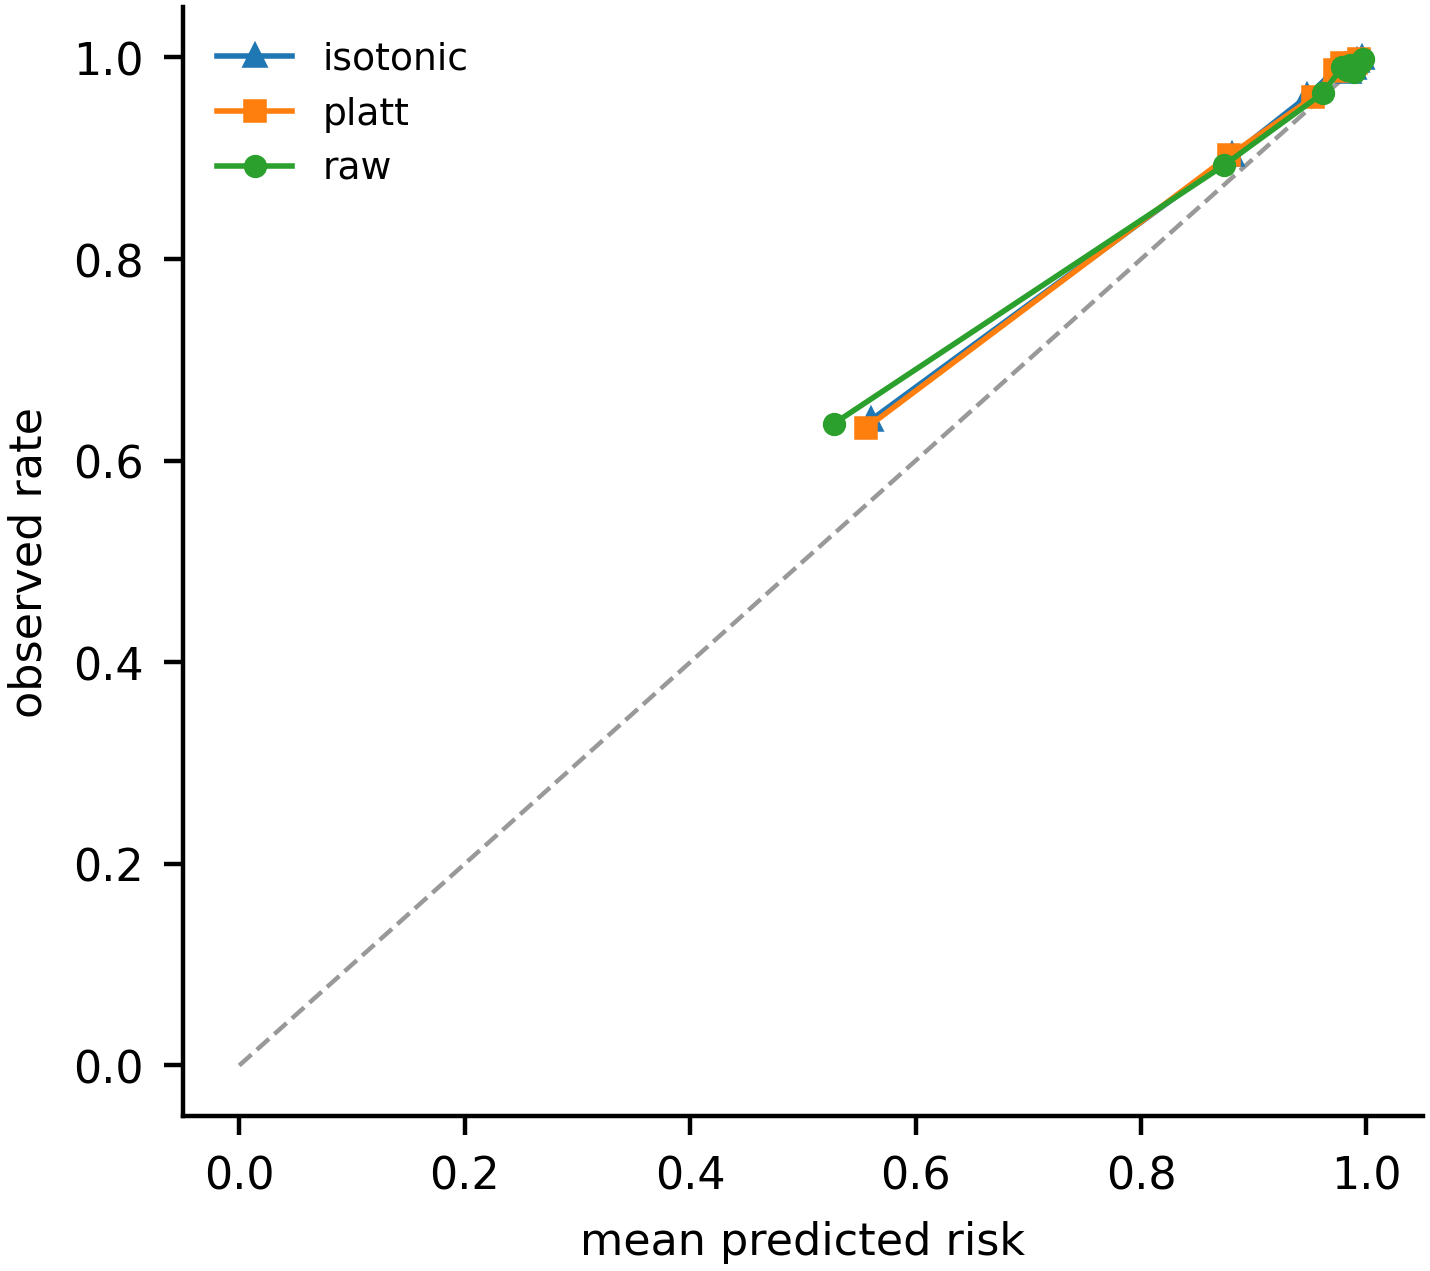
\includegraphics[width=0.72\linewidth]{figS7_calibration.png}
\caption{Calibration at the reference cell on the case study's log, by decile
of predicted risk. The two proper scoring rules on the metric axis --- Brier
skill and the log-loss skill --- read this picture; the two rank-based ones
cannot see it at all (Proposition~\ref{prop:rank}). A pipeline whose
discrimination is adequate and whose calibration is not therefore moves the
increment on some instruments and not others, which is one concrete mechanism
behind the metric axis's contribution to Table~\ref{tab:sobol}.}
\label{fig:calibration}
\end{figure}

The frequency-encoded pipeline is the one that is visibly miscalibrated, with
a slope well below one, and it is also the one whose increment differs most
from the others on the two proper scoring rules. That is the interaction
between the pipeline axis and the metric axis, drawn.

Rolling-origin results are in \texttt{results/s01\_surface.csv} under
\texttt{split = rolling$k$} and enter the decomposition as the split axis;
Supplement~\ref{app:rolling} prints them per fold. The single holdout is not
the best estimate of the increment, and reporting it alone would be a
limitation.


\section{Tables the article summarises}
\label{app:tables}
The article prints the seven tables a reader needs to follow its argument.
This section carries the ones it summarises: the exclusion ledger, the
construct audit, the surface denominator, the planned contrasts, the region
labels, the ITSM family split, the sign-flip attribution, the cohort
decomposition, the axis-kind partition, the specification-curve comparison,
the desk utility, the tipping curve, the decision-curve corpus, the declared
measures, the four decision rules, the calibration diagnostics, the
availability evidence, the severity sweeps, the absorption ladders, and the
simulation in full. Every one is generated by
\texttt{scripts/make\_numbers.py} from the result files, and none is typed by
hand.

\subsection{The corpus}

\begin{table}[t]
\centering
\small
\resizebox{\ifdim\width>\linewidth\linewidth\else\width\fi}{!}{%%
\begin{tabular}{llll}
\toprule
log & domain & code & detail \\
\midrule
Helpdesk & itsm & NO\_HEADROOM & handover/primary prev=0.9993 \\
Helpdesk & itsm & NO\_HEADROOM & handover/g=workgroup prev=0.0011 \\
BPIC13\_open & itsm & SMALL\_N & n=819 \\
BPIC13\_closed & itsm & NO\_TEST\_VARIATION & duration \\
BPIC12 & lending & NO\_G & n=13087 \\
BPIC17 & lending & NO\_HEADROOM & handover/primary prev=0.9977 \\
BPIC19 & procurement & NO\_HEADROOM & handover/primary prev=0.9631 \\
BPIC15\_2 & permitting & SMALL\_N & n=832 \\
BPIC15\_5 & permitting & NO\_HEADROOM & handover/primary prev=0.9593 \\
BPIC20\_domestic & expenses & NO\_G & n=10500 \\
BPIC20\_intl & expenses & NO\_G & n=6449 \\
BPIC20\_prepaid & expenses & NO\_G & n=2099 \\
BPIC20\_permit & expenses & NO\_G & n=7065 \\
BPIC20\_rfp & expenses & NO\_G & n=6886 \\
Sepsis & healthcare & NO\_HEADROOM & handover/primary prev=1.0000 \\
HospitalBilling & healthcare & NO\_F & n=100000 \\
RoadFines & enforcement & NO\_HEADROOM & handover/primary prev=0.0037 \\
BPIC11 & healthcare & HELD\_OUT & downloaded as a held-out log for the out-of-corpus test; never offered to the admission rules \\
BPIC18 & agriculture & NO\_TEST\_VARIATION & held-out set: duration \\
BPIC18 & agriculture & NO\_HEADROOM & held-out set: handover prev=1.0000 \\
\bottomrule
\end{tabular}%
}
\caption{Every downloaded log that is not among the \nPairs\ admitted log--target pairs, with its registered exclusion code. \textsf{HELD\_OUT} names the logs downloaded as a held-out set for a separate test and never offered to the admission rules; every other code is a rule of Section~\ref{sec:design}. Some logs appear here under one target and among the admitted pairs under the other, which is what a per-pair admission rule does.}
\label{tab:corpus}
\end{table}


\begin{table}[t]
\centering
\footnotesize
\setlength{\tabcolsep}{5pt}%
\renewcommand{\arraystretch}{1.15}%
\hyphenpenalty=50 \exhyphenpenalty=50 \emergencystretch=1em\relax%
\resizebox{\ifdim\width>\linewidth\linewidth\else\width\fi}{!}{%%
\begin{tabular}{lllll>{\raggedright\arraybackslash}p{0.200\linewidth}>{\raggedright\arraybackslash}p{0.200\linewidth}}
\toprule
log & domain & target & register & free field & why it behaves as a register & threat to construct validity \\
\midrule
RoadFines & enforcement & duration & article & org:resource & article of law, reused across fines & semantics legal, not operational \\
Sepsis & healthcare & duration & Diagnose & org:group & diagnosis vocabulary: reused, not maintained & no maintenance process; quality axis hypothetical \\
BPIC13\_closed & itsm & handover & product & org:resource & maintained CI or customer register & none beyond domain: closest to the case study \\
BPIC13\_incidents & itsm & duration & product & org:resource & maintained CI or customer register & none beyond domain: closest to the case study \\
BPIC13\_incidents & itsm & handover & product & org:resource & maintained CI or customer register & none beyond domain: closest to the case study \\
BPIC14 & itsm & duration & CI Name (aff) & assignment group & maintained CI or customer register & none beyond domain: closest to the case study \\
BPIC14 & itsm & handover & CI Name (aff) & assignment group & maintained CI or customer register & none beyond domain: closest to the case study \\
Helpdesk & itsm & duration & customer & Resource & maintained CI or customer register & none beyond domain: closest to the case study \\
UCI498 & itsm & duration & caller\_id & assigned\_to & maintained CI or customer register & none beyond domain: closest to the case study \\
UCI498 & itsm & handover & caller\_id & assigned\_to & maintained CI or customer register & none beyond domain: closest to the case study \\
BPIC17 & lending & duration & case:RequestedAmount & org:resource & application or offer reference & near-unique per case, so reuse is thin \\
BPIC15\_1 & permitting & duration & case:parts & org:resource & case-type reference, reused & nobody curates it \\
BPIC15\_1 & permitting & handover & case:parts & org:resource & case-type reference, reused & nobody curates it \\
BPIC15\_3 & permitting & duration & case:parts & org:resource & case-type reference, reused & nobody curates it \\
BPIC15\_3 & permitting & handover & case:parts & org:resource & case-type reference, reused & nobody curates it \\
BPIC15\_4 & permitting & duration & case:parts & org:resource & case-type reference, reused & nobody curates it \\
BPIC15\_4 & permitting & handover & case:parts & org:resource & case-type reference, reused & nobody curates it \\
BPIC15\_5 & permitting & duration & case:parts & org:resource & case-type reference, reused & nobody curates it \\
BPIC19 & procurement & duration & case:Vendor & org:resource & item or vendor catalogue entry & target is a duration, not a routing decision \\
\bottomrule
\end{tabular}%
}
\caption{Construct validity, per log--target pair: the field playing the register role, why it behaves as a maintained and reused entity, the free field, and the specific threat to construct validity the pair carries. These are not the same construct, which is why the corpus is a benchmark of specification sensitivity rather than a replication.}
\label{tab:construct}
\end{table}


\begin{table}[t]
\centering
\small
\resizebox{\ifdim\width>\linewidth\linewidth\else\width\fi}{!}{%%
\begin{tabular}{lllllllllllllllr}
\toprule
log & target & learners & splits & quality & rungs & metrics & declared scalar & computed scalar & model fits & duplicates & missing & inference cells & draws & register levels K & K / n train \\
\midrule
BPIC13\_closed & handover & 2 & 6 & 6 & 3 & 5 & 1080 & 1080 & 288 & 0 & 0 & 36 & 400 & 337 & 0.324 \\
BPIC13\_incidents & duration & 2 & 6 & 6 & 3 & 5 & 1080 & 1080 & 288 & 0 & 0 & 36 & 400 & 704 & 0.133 \\
BPIC13\_incidents & handover & 2 & 6 & 6 & 3 & 5 & 1080 & 1080 & 288 & 0 & 0 & 36 & 400 & 704 & 0.133 \\
BPIC14 & duration & 4 & 6 & 10 & 4 & 5 & 4800 & 4800 & 1200 & 0 & 0 & 36 & 400 & 3019 & 0.093 \\
BPIC14 & handover & 4 & 6 & 10 & 4 & 5 & 4800 & 4800 & 1200 & 0 & 0 & 36 & 400 & 3019 & 0.093 \\
BPIC15\_1 & duration & 2 & 6 & 6 & 3 & 5 & 1080 & 1080 & 288 & 0 & 0 & 36 & 400 & 89 & 0.106 \\
BPIC15\_1 & handover & 2 & 6 & 6 & 3 & 5 & 1080 & 1080 & 288 & 0 & 0 & 36 & 400 & 89 & 0.106 \\
BPIC15\_3 & duration & 2 & 6 & 6 & 3 & 5 & 1080 & 1080 & 288 & 0 & 0 & 36 & 400 & 94 & 0.095 \\
BPIC15\_3 & handover & 2 & 6 & 6 & 3 & 5 & 1080 & 1080 & 288 & 0 & 0 & 36 & 400 & 94 & 0.095 \\
BPIC15\_4 & duration & 2 & 6 & 6 & 3 & 5 & 1080 & 1080 & 288 & 0 & 0 & 36 & 400 & 53 & 0.072 \\
BPIC15\_4 & handover & 2 & 6 & 6 & 3 & 5 & 1080 & 1080 & 288 & 0 & 0 & 36 & 400 & 53 & 0.072 \\
BPIC15\_5 & duration & 2 & 6 & 6 & 3 & 5 & 1080 & 1080 & 288 & 0 & 0 & 36 & 400 & 107 & 0.132 \\
BPIC17 & duration & 2 & 6 & 6 & 3 & 5 & 1080 & 1080 & 288 & 0 & 0 & 36 & 400 & 701 & 0.032 \\
BPIC19 & duration & 3 & 6 & 6 & 3 & 5 & 1620 & 1620 & 432 & 0 & 0 & 36 & 400 & 1975 & 0.011 \\
Helpdesk & duration & 2 & 6 & 6 & 3 & 5 & 1080 & 1080 & 288 & 0 & 0 & 36 & 400 & 394 & 0.123 \\
RoadFines & duration & 3 & 6 & 6 & 3 & 5 & 1620 & 1620 & 432 & 0 & 0 & 36 & 400 & 66 & 0.001 \\
Sepsis & duration & 2 & 6 & 6 & 3 & 5 & 1080 & 1080 & 288 & 0 & 0 & 36 & 400 & 147 & 0.200 \\
UCI498 & duration & 2 & 6 & 6 & 3 & 5 & 1080 & 1080 & 288 & 0 & 0 & 36 & 400 & 5245 & 0.301 \\
UCI498 & handover & 2 & 6 & 6 & 3 & 5 & 1080 & 1080 & 288 & 0 & 0 & 36 & 400 & 5245 & 0.301 \\
\bottomrule
\end{tabular}%
}
\caption{The surface denominator audit. For every log--target pair: the declared level count on each axis, then two counts \emph{on the same basis} --- the admissible scalar cells the declaration multiplies out, and the same cells counted in the surface file --- which are equal on every pair. `model fits' is a different quantity and is printed separately: it counts fitted arms before the expansion over instruments and \emph{includes} the intercept-only rung, which the master surface carries so that the surface is complete and which no admissible set contains. Then duplicates, missing combinations, the size and draw count of the inference surface, the register's cardinality and its ratio to the training row count, which Section~\ref{sec:simsensitivity} shows is what governs whether the bands cover at their nominal level.}
\label{tab:denominator}
\end{table}


\begin{table}[t]\centering\small
\textbf{??} this table's source has not been generated yet.
\caption{Confirmatory contrasts.}\label{tab:confirm}\end{table}


\subsection{Regions, sign flips and the cohort decomposition}

\begin{table}[t]
\centering
\small
\resizebox{\ifdim\width>\linewidth\linewidth\else\width\fi}{!}{%%
\begin{tabular}{llllllrlrl}
\toprule
log & target & cells & beneficial & harmful & unresolved & rho & region & q & label under the narrow family \\
\midrule
BPIC13\_closed & handover & 180 & 0 & 1 & 179 & -0.006 & conditionally harmful & 3.338 & sign-changing \\
BPIC13\_incidents & duration & 180 & 21 & 0 & 159 & 0.117 & conditionally beneficial & 3.354 & sign-changing \\
BPIC13\_incidents & handover & 180 & 97 & 0 & 83 & 0.539 & conditionally beneficial & 3.330 & conditionally beneficial \\
BPIC14 & duration & 480 & 337 & 0 & 143 & 0.702 & conditionally beneficial & 3.492 & conditionally beneficial \\
BPIC14 & handover & 480 & 279 & 2 & 199 & 0.577 & sign-changing & 3.569 & sign-changing \\
BPIC15\_1 & duration & 180 & 6 & 0 & 174 & 0.033 & conditionally beneficial & 3.339 & conditionally beneficial \\
BPIC15\_1 & handover & 180 & 2 & 0 & 178 & 0.011 & conditionally beneficial & 3.358 & sign-changing \\
BPIC15\_3 & duration & 180 & 40 & 0 & 140 & 0.222 & conditionally beneficial & 3.335 & sign-changing \\
BPIC15\_3 & handover & 180 & 2 & 0 & 178 & 0.011 & conditionally beneficial & 3.318 & sign-changing \\
BPIC15\_4 & duration & 180 & 0 & 0 & 180 & 0.000 & unresolved & 3.380 & sign-changing \\
BPIC15\_4 & handover & 180 & 0 & 0 & 180 & 0.000 & unresolved & 3.425 & sign-changing \\
BPIC15\_5 & duration & 180 & 4 & 3 & 173 & 0.006 & sign-changing & 3.395 & sign-changing \\
BPIC17 & duration & 180 & 35 & 0 & 145 & 0.194 & conditionally beneficial & 3.252 & conditionally beneficial \\
BPIC19 & duration & 120 & 14 & 28 & 78 & -0.117 & sign-changing & 3.317 & sign-changing \\
Helpdesk & duration & 180 & 0 & 8 & 172 & -0.044 & conditionally harmful & 3.312 & sign-changing \\
RoadFines & duration & 120 & 47 & 20 & 53 & 0.225 & sign-changing & 3.140 & sign-changing \\
Sepsis & duration & 180 & 106 & 0 & 74 & 0.589 & conditionally beneficial & 3.320 & conditionally beneficial \\
UCI498 & duration & 180 & 58 & 0 & 122 & 0.322 & conditionally beneficial & 3.257 & conditionally beneficial \\
UCI498 & handover & 180 & 40 & 0 & 140 & 0.222 & conditionally beneficial & 3.329 & sign-changing \\
\bottomrule
\end{tabular}%
}
\caption{Resolution regions from the WHOLE-SURFACE simultaneous band at its NOMINAL critical value, with that value $q$ and, for comparison, the label a narrower within-instrument family would have given the same draws. \textbf{These are not the labels the article quotes}: the article's regions and $\rho$ are computed under the coverage-calibrated critical value and are in Table~\ref{tab:calbands}. This table is printed so that the cost of the wider FAMILY is visible separately from the cost of the CALIBRATION.}
\label{tab:regions}
\end{table}


\begin{table}[t]
\centering
\footnotesize
\setlength{\tabcolsep}{5pt}%
\renewcommand{\arraystretch}{1.15}%
\hyphenpenalty=50 \exhyphenpenalty=50 \emergencystretch=1em\relax%
\resizebox{\ifdim\width>\linewidth\linewidth\else\width\fi}{!}{%%
\begin{tabular}{>{\raggedright\arraybackslash}p{0.260\linewidth}>{\raggedright\arraybackslash}p{0.200\linewidth}>{\raggedright\arraybackslash}p{0.200\linewidth}>{\raggedright\arraybackslash}p{0.200\linewidth}}
\toprule
statistic & all 19 & itsm 8 & other 11 \\
\midrule
baseline spread (AUC) & 0.073 [0.024, 0.097] & 0.070 [0.014, 0.132] & 0.088 [0.022, 0.097] \\
higher-order share & 0.560 [0.409, 0.608] & 0.365 [0.233, 0.450] & 0.608 [0.532, 0.732] \\
largest first-order index & 0.287 [0.185, 0.352] & 0.355 [0.278, 0.358] & 0.201 [0.151, 0.305] \\
misreport, all cells & 0.328 [0.243, 0.452] & 0.271 [0.244, 0.481] & 0.353 [0.191, 0.617] \\
misreport, analyst latitude only & 0.200 [0.100, 0.467] & 0.194 [0.067, 0.367] & 0.400 [0.067, 0.600] \\
misreport, magnitude-weighted & 0.502 [0.102, 0.623] & 0.296 [0.025, 0.623] & 0.507 [0.139, 0.640] \\
misreport, resolved cells (pooled) & 0.075 & 0.035 & 0.222 \\
robustness index rho (calibrated) & 0.017 [0.000, 0.182] & 0.069 [-0.006, 0.552] & 0.000 [0.000, 0.182] \\
one-number excess regret (AUC) & 0.000 [0.000, 0.003] & 0.000 [0.000, 0.011] & 0.000 [0.000, 0.005] \\
\bottomrule
\end{tabular}%
}
\caption{Every headline corpus statistic on three populations: all nineteen log--target pairs, the eight from IT service management where the register is a maintained configuration or customer register, and the eleven where it is not. Each cell is the statistic with a 95\% percentile interval from a cluster bootstrap that resamples LOGS, because two targets on the same log share a cohort and are not two independent observations. The resolved-cell row is a pooled ratio --- disagreeing cells over resolved cells, summed across the population --- and not a median of per-pair rates, which on a population where most pairs resolve little prints zero and says nothing.}
\label{tab:family}
\end{table}


\begin{table}[t]
\centering
\small
\begin{tabular}{llrrrrr}
\toprule
log & target & learner & metric & quality & rung & split \\
\midrule
BPIC13\\_closed & handover & 0.287 & 0.214 & 0.234 & 0.222 & 0.401 \\
BPIC13\\_incidents & duration & 0.374 & 0.249 & 0.204 & 0.230 & 0.405 \\
BPIC13\\_incidents & handover & 0.174 & 0.089 & 0.111 & 0.100 & 0.181 \\
BPIC14 & duration & 0.155 & 0.051 & 0.121 & 0.150 & 0.089 \\
BPIC14 & handover & 0.426 & 0.096 & 0.115 & 0.139 & 0.113 \\
BPIC15\\_1 & duration & 0.383 & 0.217 & 0.228 & 0.348 & 0.446 \\
BPIC15\\_1 & handover & 0.313 & 0.168 & 0.232 & 0.263 & 0.331 \\
BPIC15\\_3 & duration & 0.337 & 0.144 & 0.164 & 0.187 & 0.250 \\
BPIC15\\_3 & handover & 0.365 & 0.302 & 0.217 & 0.276 & 0.449 \\
BPIC15\\_4 & duration & 0.431 & 0.169 & 0.238 & 0.196 & 0.501 \\
BPIC15\\_4 & handover & 0.450 & 0.254 & 0.255 & 0.287 & 0.454 \\
BPIC15\\_5 & duration & 0.426 & 0.194 & 0.221 & 0.309 & 0.335 \\
BPIC17 & duration & 0.291 & 0.219 & 0.257 & 0.224 & 0.397 \\
BPIC19 & duration & 0.035 & 0.235 & 0.090 & 0.052 & 0.447 \\
Helpdesk & duration & 0.252 & 0.273 & 0.181 & 0.131 & 0.284 \\
RoadFines & duration & 0.043 & 0.143 & 0.194 & 0.056 & 0.178 \\
Sepsis & duration & 0.113 & 0.066 & 0.058 & 0.063 & 0.089 \\
UCI498 & duration & 0.300 & 0.197 & 0.199 & 0.383 & 0.384 \\
UCI498 & handover & 0.333 & 0.206 & 0.230 & 0.489 & 0.289 \\
\bottomrule
\end{tabular}

\caption{Sign flips attributable to each axis: the share of pairs of cells that agree on every other axis and disagree on the sign of the increment.}
\label{tab:regret}
\end{table}


\begin{table}[t]
\centering
\small
\resizebox{\ifdim\width>\linewidth\linewidth\else\width\fi}{!}{%%
\begin{tabular}{lrrr}
\toprule
effect & B intake & B intake g & B intake g km \\
\midrule
cohort & 0.000 & 0.000 & 0.000 \\
cohort x target & 0.000 & 0.000 & 0.007 \\
target & 1.000 & 1.000 & 0.993 \\
\bottomrule
\end{tabular}%
}
\caption{The exact two-factor decomposition of the discrepancy. Share of the variance of $V$ over the cohort $\times$ target design, at each rung of the ladder, at a declared tie-break. With two levels per factor the decomposition is exact.}
\label{tab:cohortanova}
\end{table}


\begin{table}[t]
\centering
\small
\resizebox{\ifdim\width>\linewidth\linewidth\else\width\fi}{!}{%%
\begin{tabular}{llrrrr}
\toprule
log & target & analyst latitude & resampling & counterfactual & higher-order \\
\midrule
BPIC13\_closed & handover & 0.223 & 0.203 & 0.029 & 0.546 \\
BPIC13\_incidents & duration & 0.111 & 0.384 & 0.029 & 0.475 \\
BPIC13\_incidents & handover & 0.174 & 0.172 & 0.099 & 0.555 \\
BPIC14 & duration & 0.606 & 0.013 & 0.151 & 0.231 \\
BPIC14 & handover & 0.631 & 0.010 & 0.127 & 0.232 \\
BPIC15\_1 & duration & 0.084 & 0.263 & 0.039 & 0.613 \\
BPIC15\_1 & handover & 0.106 & 0.079 & 0.036 & 0.779 \\
BPIC15\_3 & duration & 0.037 & 0.287 & 0.081 & 0.595 \\
BPIC15\_3 & handover & 0.128 & 0.189 & 0.004 & 0.679 \\
BPIC15\_4 & duration & 0.083 & 0.111 & 0.025 & 0.781 \\
BPIC15\_4 & handover & 0.090 & 0.050 & 0.031 & 0.829 \\
BPIC15\_5 & duration & 0.157 & 0.036 & 0.042 & 0.766 \\
BPIC17 & duration & 0.001 & 0.346 & 0.062 & 0.591 \\
BPIC19 & duration & 0.017 & 0.491 & 0.011 & 0.481 \\
Helpdesk & duration & 0.287 & 0.222 & 0.086 & 0.405 \\
RoadFines & duration & 0.065 & 0.192 & 0.289 & 0.454 \\
Sepsis & duration & 0.127 & 0.134 & 0.145 & 0.594 \\
UCI498 & duration & 0.107 & 0.399 & 0.030 & 0.465 \\
UCI498 & handover & 0.396 & 0.136 & 0.071 & 0.398 \\
\bottomrule
\end{tabular}%
}
\caption{The variance decomposition partitioned by what KIND of choice each axis is. \emph{Analyst latitude} is the pipeline, the baseline rung and the instrument --- things an analyst chooses and could have chosen otherwise. \emph{Resampling} is the split, five of whose six levels are expanding-origin folds on the same data and are therefore different samples rather than different analyses. \emph{Counterfactual} is the register-quality condition, which is a different state of the world. The remainder belongs to no single axis. A reader asking what a one-number report exposes them to should read the first column.}
\label{tab:axiskind}
\end{table}


\begin{table}[t]
\centering
\small
\resizebox{\ifdim\width>\linewidth\linewidth\else\width\fi}{!}{%%
\begin{tabular}{lllrrrrrllr}
\toprule
log & target & cases & capped & observed median & null median & p (median) & share positive & SCA verdict & region & rho \\
\midrule
BPIC13\_closed & handover & 1487 & False & -0.010 & -0.008 & 0.327 & 0.208 & not distinguishable from null & unresolved & 0.000 \\
BPIC13\_incidents & duration & 7554 & False & 0.010 & -0.012 & 0.673 & 0.625 & not distinguishable from null & conditionally beneficial & 0.017 \\
BPIC13\_incidents & handover & 7554 & False & 0.031 & -0.006 & 0.010 & 0.833 & non-null at 5\% & conditionally beneficial & 0.400 \\
BPIC14 & duration & 20000 & True & 0.091 & -0.001 & 0.010 & 1.000 & non-null at 5\% & conditionally beneficial & 0.692 \\
BPIC14 & handover & 20000 & True & 0.035 & 0.000 & 0.010 & 0.750 & non-null at 5\% & sign-changing & 0.552 \\
BPIC15\_1 & duration & 1199 & False & 0.030 & 0.001 & 0.010 & 0.792 & non-null at 5\% & conditionally beneficial & 0.011 \\
BPIC15\_1 & handover & 1199 & False & 0.002 & -0.002 & 0.653 & 0.708 & not distinguishable from null & unresolved & 0.000 \\
BPIC15\_3 & duration & 1409 & False & 0.119 & 0.003 & 0.010 & 0.958 & non-null at 5\% & conditionally beneficial & 0.056 \\
BPIC15\_3 & handover & 1409 & False & 0.023 & -0.005 & 0.020 & 0.625 & non-null at 5\% & unresolved & 0.000 \\
BPIC15\_4 & duration & 1053 & False & -0.030 & -0.004 & 0.010 & 0.333 & non-null at 5\% & unresolved & 0.000 \\
BPIC15\_4 & handover & 1053 & False & -0.018 & -0.011 & 0.158 & 0.250 & not distinguishable from null & unresolved & 0.000 \\
BPIC15\_5 & duration & 1156 & False & 0.043 & -0.001 & 0.010 & 0.833 & non-null at 5\% & unresolved & 0.000 \\
BPIC17 & duration & 20000 & True & 0.006 & -0.001 & 0.030 & 0.708 & non-null at 5\% & conditionally beneficial & 0.139 \\
BPIC19 & duration & 20000 & True & 0.051 & -0.001 & 0.010 & 1.000 & non-null at 5\% & sign-changing & -0.083 \\
Helpdesk & duration & 4580 & False & -0.013 & -0.008 & 0.109 & 0.208 & not distinguishable from null & conditionally harmful & -0.011 \\
RoadFines & duration & 20000 & True & 0.016 & 0.000 & 0.010 & 0.792 & non-null at 5\% & sign-changing & 0.225 \\
Sepsis & duration & 1050 & False & 0.154 & -0.003 & 0.010 & 1.000 & non-null at 5\% & conditionally beneficial & 0.283 \\
UCI498 & duration & 20000 & True & 0.005 & -0.005 & 0.396 & 0.625 & not distinguishable from null & conditionally beneficial & 0.094 \\
UCI498 & handover & 20000 & True & 0.000 & -0.002 & 1.000 & 0.500 & not distinguishable from null & conditionally beneficial & 0.044 \\
\bottomrule
\end{tabular}%
}
\caption{Specification-curve analysis as practised, beside this paper's region label. The permutation test asks whether the surface as a whole differs from one with no signal in it; the region asks, of each cell, whether the sign of that cell's own increment is determined. Where the two part company is what the extra machinery is for. Both verdicts are computed on the declared \nScaCells-cell sub-surface at \nScaPerms\ permutations; `cases' is the number of cases the permutation test ran on, which is the pair's own count unless the declared cap of \nScaMaxCases\ bound on it. The region column is the coverage-calibrated label of Section~\ref{sec:regions}, computed on the full data.}
\label{tab:sca}
\end{table}


\begin{table}[t]
\centering
\small
\resizebox{\ifdim\width>\linewidth\linewidth\else\width\fi}{!}{%%
\begin{tabular}{lllrll}
\toprule
threshold measure & majority & one-number & uniform-beneficial & weighted-mean & pairs where the rules differ \\
\midrule
desk distribution & 0 & 0 & 0.0477 & 0 & 11 \\
fixed 1:19 & 0 & 0 & 0.0000 & 0 & 5 \\
fixed 1:2 & 0 & 0 & 0.3251 & 0 & 10 \\
fixed 1:4 & 0 & 0 & 0.2127 & 0 & 11 \\
fixed 1:9 & 0 & 0 & 0.0000 & 0 & 7 \\
uniform over the declared range & 0 & 0 & 1.3468 & 0 & 13 \\
\bottomrule
\end{tabular}%
}
\caption{Median excess regret of each decision rule, in net benefit per thousand cases, on the models that pass the registered calibration rule. The desk distribution places its mass on the exchange rates a service desk plausibly holds; the fixed rows report single exchange rates so that a reader who rejects the distribution still has a number. The last column counts the pairs on which the four rules do not all lose the same, out of the \nPairsDesk\ pairs that carry a model the calibration rule admits --- NOT out of \nPairs: the rule excludes \nPairsDcaExcluded\ of them, and a count taken over the admitted pairs and printed against the corpus total is the defect this caption exists to prevent.}
\label{tab:desk}
\end{table}


\begin{table}[t]\centering\small
\textbf{??} this table's source has not been generated yet.
\caption{Leakage tipping point.}\label{tab:tipping}\end{table}


\begin{table}[t]\centering\small
\textbf{??} this table's source has not been generated yet.
\caption{Decision curve.}\label{tab:dca}\end{table}


\subsection{Measures, rules and calibration}

\begin{table}[t]
\centering
\small
\resizebox{\ifdim\width>\linewidth\linewidth\else\width\fi}{!}{%%
\begin{tabular}{llrrrrll}
\toprule
measure & description & median & min & max & largest first order median & n pairs first order exceeds & n pairs \\
\midrule
equal-level & every level of every axis equally likely & 0.560 & 0.233 & 0.793 & 0.287 & 6 & 19 \\
reference & half the mass on the reference level of each axis & 0.496 & 0.157 & 0.709 & 0.299 & 6 & 19 \\
concentrated & eighty per cent on the reference level & 0.317 & 0.065 & 0.638 & 0.392 & 12 & 19 \\
envelope & 200 Dirichlet draws of the level weights, primary pair & 0.181 & 0.098 & 0.347 & -- & -- & -- \\
\bottomrule
\end{tabular}%
}
\caption{The declared measures over specifications, and the total higher-order variance share under each. `largest first order median' is the median over pairs of the largest single first-order index under the same measure, and `n pairs first order exceeds' counts the pairs on which that index is LARGER than the higher-order total. THE MAGNITUDE MOVES WITH THE MEASURE, AND SO DOES THE QUALITATIVE CONCLUSION: across the three product measures the higher-order share moves by \measureSpreadPct, and under the measure concentrated on the reference level it is \interactionTotalConcentratedPct, BELOW the largest first-order index of \concentratedFirstOrderPct, with a first-order index exceeding the higher-order remainder on \nConcentratedExceeds\ of \nPairs\ pairs --- and on \nEqualExceeds\ of \nPairs\ even under the primary equal-level measure. `The interactions carry more than any main effect' is therefore a claim about a measure and not only about a surface, and Section~\ref{sec:axes2} states it as one. The envelope row is the Dirichlet envelope on the primary pair alone, so it carries no corpus-wide comparison and its last three cells are dashes rather than zeroes.}
\label{tab:measures}
\end{table}


\begin{table}[t]
\centering
\small
\begin{tabular}{lrr}
\toprule
rule & reference-adjacent & uniform \\
\midrule
majority & 0.020 & 0.030 \\
one-number & 0.024 & 0.038 \\
uniform-beneficial & 0.045 & 0.049 \\
\bottomrule
\end{tabular}

\caption{Three decision rules under one loss: the mean regret per log--target pair, in the metric's own units, under a uniform draw over the admissible set and under a draw concentrated near the conventional specification.}
\label{tab:rules}
\end{table}


\begin{table}[t]
\centering
\small
\resizebox{\ifdim\width>\linewidth\linewidth\else\width\fi}{!}{%%
\begin{tabular}{llllrrrrr}
\toprule
log & target & n train & n test & prev test & cal intercept & cal slope & brier & unseen \\
\midrule
BPIC13\_closed & handover & 1040 & 447 & 0.275 & -0.368 & 0.916 & 0.170 & 0.407 \\
BPIC13\_incidents & duration & 5287 & 2267 & 0.154 & -1.783 & 0.571 & 0.216 & 0.105 \\
BPIC13\_incidents & handover & 5287 & 2267 & 0.616 & -0.925 & 0.943 & 0.167 & 0.105 \\
BPIC15\_1 & duration & 839 & 360 & 0.442 & -1.204 & 0.997 & 0.228 & 0.753 \\
BPIC15\_1 & handover & 839 & 360 & 0.839 & -0.061 & 1.255 & 0.066 & 0.753 \\
BPIC15\_3 & duration & 986 & 423 & 0.456 & -0.746 & 0.928 & 0.214 & 0.095 \\
BPIC15\_3 & handover & 986 & 423 & 0.905 & -0.649 & 1.437 & 0.069 & 0.095 \\
BPIC15\_4 & duration & 737 & 316 & 0.225 & -1.927 & 0.029 & 0.351 & 0.649 \\
BPIC15\_4 & handover & 737 & 316 & 0.867 & -1.349 & 0.302 & 0.119 & 0.649 \\
BPIC15\_5 & duration & 809 & 347 & 0.285 & -0.793 & 0.290 & 0.244 & 0.867 \\
BPIC17 & duration & 22056 & 9453 & 0.494 & -0.060 & 0.758 & 0.244 & 0.060 \\
BPIC14 & handover & 32624 & 13982 & 0.945 & 0.378 & 0.994 & 0.037 & 0.053 \\
Helpdesk & duration & 3206 & 1374 & 0.451 & -0.149 & 0.475 & 0.245 & 0.229 \\
Sepsis & duration & 735 & 315 & 0.444 & -0.307 & 0.716 & 0.192 & 0.079 \\
BPIC14 & duration & 32624 & 13982 & 0.427 & -0.259 & 0.938 & 0.202 & 0.053 \\
UCI498 & duration & 17442 & 7476 & 0.286 & -0.619 & 0.811 & 0.176 & 0.192 \\
RoadFines & duration & 105259 & 45111 & 0.429 & -0.312 & 0.626 & 0.244 & 0.368 \\
UCI498 & handover & 17442 & 7476 & 0.420 & 0.017 & 1.230 & 0.071 & 0.192 \\
BPIC19 & duration & 176213 & 75521 & 0.162 & -3.163 & 0.278 & 0.352 & 0.299 \\
\bottomrule
\end{tabular}%
}
\caption{Calibration and unseen-category rates at the reference cell.}
\label{tab:calibration}
\end{table}


\begin{table}[t]
\centering
\small
\resizebox{\ifdim\width>\linewidth\linewidth\else\width\fi}{!}{%%
\begin{tabular}{llrrrrrr}
\toprule
log & target & raw slope & platt slope & isotonic slope & raw ece & platt ece & isotonic ece \\
\midrule
BPIC13\_closed & handover & 0.332 & 1.005 & 0.886 & 0.149 & 0.120 & 0.096 \\
BPIC13\_incidents & duration & 0.575 & 1.052 & 0.902 & 0.295 & 0.304 & 0.296 \\
BPIC13\_incidents & handover & 0.743 & 1.334 & 1.049 & 0.140 & 0.149 & 0.142 \\
BPIC14 & duration & 0.945 & 1.117 & 1.050 & 0.056 & 0.056 & 0.056 \\
BPIC14 & handover & 0.952 & 1.049 & 0.995 & 0.017 & 0.015 & 0.015 \\
BPIC15\_1 & duration & 0.731 & 1.812 & 1.118 & 0.208 & 0.172 & 0.152 \\
BPIC15\_1 & handover & 0.778 & 1.654 & 1.466 & 0.075 & 0.066 & 0.050 \\
BPIC15\_3 & duration & 0.886 & 1.225 & 1.109 & 0.190 & 0.152 & 0.152 \\
BPIC15\_3 & handover & 0.450 & 1.247 & 0.904 & 0.071 & 0.057 & 0.039 \\
BPIC15\_4 & duration & 0.025 & 0.028 & $-$0.013 & 0.364 & 0.313 & 0.340 \\
BPIC15\_4 & handover & 0.282 & 0.701 & 0.456 & 0.086 & 0.071 & 0.080 \\
BPIC15\_5 & duration & 0.263 & 0.853 & 0.414 & 0.252 & 0.209 & 0.211 \\
BPIC17 & duration & 0.868 & 1.165 & 1.031 & 0.023 & 0.019 & 0.017 \\
BPIC19 & duration & 0.293 & 0.355 & 0.372 & 0.339 & 0.338 & 0.338 \\
Helpdesk & duration & 0.490 & 0.731 & 0.622 & 0.088 & 0.066 & 0.065 \\
RoadFines & duration & 0.688 & 0.720 & 1.377 & 0.081 & 0.086 & 0.081 \\
Sepsis & duration & 0.456 & 0.830 & 0.554 & 0.147 & 0.086 & 0.089 \\
UCI498 & duration & 0.882 & 1.534 & 1.333 & 0.104 & 0.185 & 0.175 \\
UCI498 & handover & 1.077 & 1.453 & 1.203 & 0.041 & 0.063 & 0.047 \\
\bottomrule
\end{tabular}%
}
\caption{Calibration before and after a training-only recalibration, one row per log--target pair: the median calibration slope and expected calibration error over the arms of the baseline ladder, raw and under each calibrator. A slope far from one is a score whose thresholds are not cost ratios; only curves computed on calibrated probabilities carry a probability-threshold reading.}
\label{tab:calib2}
\end{table}


\subsection{The case study}

\begin{table}[t]
\centering
\small
\begin{tabular}{lrl}
\toprule
evidence & value & establishes \\
\midrule
interactions in the file & 147004.000 & the population the knowledge reference is written in \\
interactions that never became incidents & 94250.000 & the field is written by the service-desk process, not by the incident process \\
knowledge reference populated on those & 1.000 & the same, quantitatively \\
interactions CLOSED before the incident was opened & 5.000 & airtight pre-incident availability, on five cases, which is not enough to rest a headline on \\
interactions whose recorded handling time had elapsed before the incident was opened & 41413.000 & that the desk had worked the interaction, which is not a timestamped field-value history \\
knowledge reference populated on the joined cohort & 0.911 & coverage, not timing \\
base AUC from the knowledge reference alone & 0.648 & the field is highly predictive, which is a reason for suspicion and not for confidence \\
\bottomrule
\end{tabular}

\caption{What the interaction file establishes, and what it does not.}
\label{tab:availability}
\end{table}


\begin{table}[t]
\centering
\small
\resizebox{\ifdim\width>\linewidth\linewidth\else\width\fi}{!}{%%
\begin{tabular}{lrrrrl}
\toprule
mechanism & level & populated & V & spread over seeds & seeds \\
\midrule
clean & 1.000 & 1.000 & 0.103 & 0.000 & 1 \\
corrupt & 0.050 & 1.000 & 0.099 & 0.003 & 3 \\
corrupt & 0.150 & 1.000 & 0.086 & 0.001 & 3 \\
corrupt & 0.300 & 1.000 & 0.069 & 0.002 & 3 \\
duplicate & 0.150 & 1.000 & 0.103 & 0.001 & 3 \\
duplicate & 0.500 & 1.000 & 0.104 & 0.001 & 3 \\
duplicate & 1.000 & 1.000 & 0.102 & 0.001 & 3 \\
mask\_common & 0.500 & 0.521 & 0.071 & 0.000 & 1 \\
mask\_random & 0.500 & 0.502 & 0.068 & 0.004 & 3 \\
mask\_rare & 0.250 & 0.270 & 0.041 & 0.000 & 1 \\
mask\_rare & 0.500 & 0.505 & 0.082 & 0.000 & 1 \\
mask\_rare & 0.750 & 0.762 & 0.096 & 0.000 & 1 \\
stale & 1.000 & 0.984 & 0.103 & 0.000 & 1 \\
stale\_lag & 0.100 & 0.982 & 0.107 & 0.000 & 1 \\
stale\_lag & 0.250 & 0.972 & 0.106 & 0.000 & 1 \\
stale\_lag & 0.500 & 0.940 & 0.107 & 0.000 & 1 \\
\bottomrule
\end{tabular}%
}
\caption{Register-quality mechanisms on the case study's cohort (\nCohort\ incidents) and reassignment target, at the reference cell. `level' is the share populated for the population mechanisms, the share corrupted for accuracy, the share of identities split for reconciliation and the lag for discovery. Stochastic mechanisms are averaged over \nQualitySeeds\ seeds and the spread across seeds is printed beside the mean, because mechanism variability and sampling variability are different quantities. The corpus-cohort version of this table is in Supplement~\ref{app:tables}.}
\label{tab:quality2}
\end{table}


\begin{table}[t]
\centering
\small
\resizebox{\ifdim\width>\linewidth\linewidth\else\width\fi}{!}{%%
\begin{tabular}{lllrrrrrr}
\toprule
mechanism & levels & seeds & integral & coarse & shift & seed s.d. & V complete & V empty \\
\midrule
content & 11 & 3 & 0.049 & 0.047 & 0.001 & 0.002 & 0.085 & -0.001 \\
mask\_rare & 11 & 1 & 0.069 & 0.066 & 0.003 & 0.000 & 0.103 & -0.003 \\
propensity & 11 & 3 & 0.056 & 0.054 & 0.002 & 0.002 & 0.086 & -0.001 \\
time & 11 & 1 & 0.077 & 0.088 & 0.011 & 0.000 & 0.115 & -0.001 \\
\bottomrule
\end{tabular}%
}
\caption{Register-quality mechanisms as severity CURVES rather than points, on the case study's cohort and reassignment target. The integral is taken against a uniform measure on severity over \nCaseSweepLevels\ levels; `grid shift' is how much coarsening that grid to five levels moves it, which is the check that the summary is a property of the curve and not of the grid.}
\label{tab:quality3}
\end{table}


\begin{table}[t]
\centering
\small
\resizebox{\ifdim\width>\linewidth\linewidth\else\width\fi}{!}{%%
\begin{tabular}{llrrrrrrrrl}
\toprule
b lo & b hi & V lo & V hi & D & D lo & D hi & R & R fieller lo & R fieller hi & fieller kind \\
\midrule
B\_half & B\_intake & 0.1828 & 0.1838 & $-$0.0010 & $-$0.0049 & 0.0033 & $-$0.0056 & $-$0.0270 & 0.0156 & bounded \\
B\_half & B\_intake\_g & 0.1828 & 0.1034 & 0.0793 & 0.0619 & 0.0896 & 0.4341 & 0.3572 & 0.5127 & bounded \\
B\_half & B\_intake\_g\_km & 0.1828 & $-$0.0029 & 0.1857 & 0.1759 & 0.2025 & 1.0157 & 0.9904 & 1.0425 & bounded \\
B\_intake & B\_intake\_g & 0.1838 & 0.1034 & 0.0804 & 0.0626 & 0.0914 & 0.4372 & 0.3611 & 0.5151 & bounded \\
B\_intake & B\_intake\_g\_km & 0.1838 & $-$0.0029 & 0.1867 & 0.1773 & 0.2040 & 1.0156 & 0.9905 & 1.0422 & bounded \\
B\_intake\_g & B\_intake\_g\_km & 0.1034 & $-$0.0029 & 0.1063 & 0.0965 & 0.1308 & 1.0277 & 0.9831 & 1.0771 & bounded \\
\bottomrule
\end{tabular}%
}
\caption{Absolute absorption $D = V(f \mid B_0) - V(f \mid B_1)$ first, with its own interval, then the ratio $R$ with its Fieller set and the set's kind, on the case study's cohort and reassignment target, in ROC AUC. \nFiellerUnboundedCase\ of \nFiellerCase\ reductions across all five instruments have a set that is not a bounded interval; for those a percentile interval is not a summary of anything.}
\label{tab:absorption}
\end{table}


\subsection{The same objects on the registered cohort}

Section~\ref{sec:cohort} shows that this log gives two answers, and that the
difference is the target rather than the cohort. Section~\ref{sec:cmdb} prints
the estate's own cohort and reassignment target throughout. These are the same
objects on
the registered cohort and the handover target, so that a reader can see both
without either being the one the article quotes.

\begin{table}[t]
\centering
\small
\resizebox{\ifdim\width>\linewidth\linewidth\else\width\fi}{!}{%%
\begin{tabular}{lrrr}
\toprule
mechanism & level & populated & V \\
\midrule
clean & 1.000 & 1.000 & 0.167 \\
mask\_rare & 0.750 & 0.760 & 0.140 \\
mask\_rare & 0.500 & 0.515 & 0.104 \\
mask\_rare & 0.250 & 0.268 & 0.037 \\
mask\_random & 0.500 & 0.502 & 0.095 \\
mask\_common & 0.500 & 0.512 & 0.106 \\
corrupt & 0.050 & 1.000 & 0.153 \\
corrupt & 0.150 & 1.000 & 0.132 \\
corrupt & 0.300 & 1.000 & 0.097 \\
duplicate & 0.150 & 1.000 & 0.167 \\
duplicate & 0.500 & 1.000 & 0.165 \\
duplicate & 1.000 & 1.000 & 0.163 \\
stale & 1.000 & 0.984 & 0.167 \\
stale\_lag & 0.100 & 0.982 & 0.169 \\
stale\_lag & 0.250 & 0.971 & 0.169 \\
stale\_lag & 0.500 & 0.941 & 0.164 \\
\bottomrule
\end{tabular}%
}
\caption{Register-quality mechanisms on the REGISTERED cohort (\nRegisteredCohort\ cases) and the handover target, at the reference cell, including a discovery lag and a sweep of the two accuracy mechanisms. The case study's own cohort and target are in Table~\ref{tab:quality2}.}
\label{tab:quality2corpus}
\end{table}


\begin{table}[t]
\centering
\footnotesize
\setlength{\tabcolsep}{5pt}%
\renewcommand{\arraystretch}{1.15}%
\hyphenpenalty=50 \exhyphenpenalty=50 \emergencystretch=1em\relax%
\resizebox{\ifdim\width>\linewidth\linewidth\else\width\fi}{!}{%%
\begin{tabular}{l>{\raggedright\arraybackslash}p{0.260\linewidth}llrrrrr}
\toprule
mechanism & operational failure mode & n levels & n seeds & integral & grid shift & seed s.d. & V complete & V empty \\
\midrule
content & discovery: coverage depends on the item's type & 11 & 20 & 0.090 & 0.015 & 0.031 & 0.146 & 0.000 \\
corrupt & accuracy: a share of rows carry the wrong identity & 11 & 20 & 0.113 & 0.010 & 0.005 & 0.068 & 0.167 \\
duplicate & reconciliation: one item exists under two keys & 11 & 20 & 0.165 & 0.001 & 0.001 & 0.163 & 0.167 \\
mask\_common & population: the core identities are absent & 11 & 1 & 0.104 & 0.018 & 0.000 & 0.167 & 0.014 \\
mask\_random & population: absent independently of everything & 11 & 20 & 0.088 & 0.016 & 0.004 & 0.167 & 0.000 \\
mask\_rare & population: the long tail of identities is absent & 11 & 1 & 0.092 & 0.016 & 0.000 & 0.167 & 0.014 \\
propensity & missing where the work is unusual: a training-estimated propensity drives the missingness & 11 & 20 & 0.069 & 0.010 & 0.004 & 0.119 & 0.000 \\
time & discovery: the register was populated late & 11 & 1 & 0.105 & 0.005 & 0.000 & 0.167 & 0.000 \\
\bottomrule
\end{tabular}%
}
\caption{Register-quality mechanisms as severity CURVES rather than points, on the primary log at the reference cell. Each row gives the operational failure mode the mechanism represents, the number of severities and seeds, the integral of the increment against a uniform measure on severity, how much coarsening the severity grid by a factor of four moves that integral, the spread across seeds, and the endpoints.}
\label{tab:quality3corpus}
\end{table}


\begin{table}[t]
\centering
\small
\resizebox{\ifdim\width>\linewidth\linewidth\else\width\fi}{!}{%%
\begin{tabular}{lllrrrrrrrrl}
\toprule
metric & b lo & b hi & V lo & V hi & D & D lo & D hi & R & R fieller lo & R fieller hi & fieller kind \\
\midrule
ap & B\_half & B\_intake & 0.031 & 0.030 & 0.000 & 0.000 & 0.002 & 0.014 & $-$0.027 & 0.052 & bounded \\
ap & B\_half & B\_intake\_g & 0.031 & 0.019 & 0.012 & 0.009 & 0.016 & 0.390 & 0.276 & 0.498 & bounded \\
ap & B\_half & B\_intake\_g\_km & 0.031 & 0.001 & 0.030 & 0.026 & 0.033 & 0.976 & 0.949 & 1.004 & bounded \\
ap & B\_intake & B\_intake\_g & 0.030 & 0.019 & 0.012 & 0.008 & 0.016 & 0.381 & 0.266 & 0.492 & bounded \\
ap & B\_intake & B\_intake\_g\_km & 0.030 & 0.001 & 0.029 & 0.026 & 0.033 & 0.976 & 0.948 & 1.004 & bounded \\
ap & B\_intake\_g & B\_intake\_g\_km & 0.019 & 0.001 & 0.018 & 0.014 & 0.021 & 0.961 & 0.917 & 1.007 & bounded \\
auc & B\_half & B\_intake & 0.260 & 0.257 & 0.003 & $-$0.002 & 0.015 & 0.010 & $-$0.021 & 0.039 & bounded \\
auc & B\_half & B\_intake\_g & 0.260 & 0.167 & 0.092 & 0.064 & 0.127 & 0.356 & 0.239 & 0.469 & bounded \\
auc & B\_half & B\_intake\_g\_km & 0.260 & 0.008 & 0.252 & 0.229 & 0.272 & 0.970 & 0.946 & 0.995 & bounded \\
auc & B\_intake & B\_intake\_g & 0.257 & 0.167 & 0.090 & 0.063 & 0.126 & 0.350 & 0.229 & 0.466 & bounded \\
auc & B\_intake & B\_intake\_g\_km & 0.257 & 0.008 & 0.249 & 0.228 & 0.271 & 0.970 & 0.945 & 0.995 & bounded \\
auc & B\_intake\_g & B\_intake\_g\_km & 0.167 & 0.008 & 0.160 & 0.122 & 0.179 & 0.954 & 0.917 & 0.992 & bounded \\
brier\_skill & B\_half & B\_intake & 0.269 & 0.269 & 0.000 & $-$0.003 & 0.003 & 0.001 & $-$0.009 & 0.012 & bounded \\
brier\_skill & B\_half & B\_intake\_g & 0.269 & 0.247 & 0.022 & $-$0.006 & 0.049 & 0.081 & $-$0.026 & 0.177 & bounded \\
brier\_skill & B\_half & B\_intake\_g\_km & 0.269 & 0.004 & 0.265 & 0.229 & 0.290 & 0.985 & 0.943 & 1.028 & bounded \\
brier\_skill & B\_intake & B\_intake\_g & 0.269 & 0.247 & 0.021 & $-$0.004 & 0.049 & 0.080 & $-$0.029 & 0.177 & bounded \\
brier\_skill & B\_intake & B\_intake\_g\_km & 0.269 & 0.004 & 0.265 & 0.227 & 0.292 & 0.985 & 0.943 & 1.028 & bounded \\
brier\_skill & B\_intake\_g & B\_intake\_g\_km & 0.247 & 0.004 & 0.243 & 0.208 & 0.274 & 0.983 & 0.938 & 1.031 & bounded \\
logloss\_skill & B\_half & B\_intake & 0.321 & 0.320 & 0.001 & $-$0.002 & 0.002 & 0.003 & $-$0.004 & 0.010 & bounded \\
logloss\_skill & B\_half & B\_intake\_g & 0.321 & 0.241 & 0.080 & 0.060 & 0.102 & 0.249 & 0.188 & 0.308 & bounded \\
logloss\_skill & B\_half & B\_intake\_g\_km & 0.321 & 0.015 & 0.306 & 0.279 & 0.328 & 0.954 & 0.924 & 0.985 & bounded \\
logloss\_skill & B\_intake & B\_intake\_g & 0.320 & 0.241 & 0.079 & 0.060 & 0.101 & 0.247 & 0.186 & 0.306 & bounded \\
logloss\_skill & B\_intake & B\_intake\_g\_km & 0.320 & 0.015 & 0.305 & 0.279 & 0.329 & 0.954 & 0.924 & 0.985 & bounded \\
logloss\_skill & B\_intake\_g & B\_intake\_g\_km & 0.241 & 0.015 & 0.226 & 0.203 & 0.244 & 0.939 & 0.900 & 0.980 & bounded \\
nagelkerke & B\_half & B\_intake & 0.363 & 0.362 & 0.001 & $-$0.003 & 0.002 & 0.003 & $-$0.005 & 0.010 & bounded \\
nagelkerke & B\_half & B\_intake\_g & 0.363 & 0.266 & 0.096 & 0.073 & 0.121 & 0.266 & 0.203 & 0.326 & bounded \\
nagelkerke & B\_half & B\_intake\_g\_km & 0.363 & 0.015 & 0.348 & 0.318 & 0.372 & 0.959 & 0.932 & 0.987 & bounded \\
nagelkerke & B\_intake & B\_intake\_g & 0.362 & 0.266 & 0.096 & 0.074 & 0.121 & 0.264 & 0.201 & 0.324 & bounded \\
nagelkerke & B\_intake & B\_intake\_g\_km & 0.362 & 0.015 & 0.347 & 0.318 & 0.372 & 0.959 & 0.932 & 0.987 & bounded \\
nagelkerke & B\_intake\_g & B\_intake\_g\_km & 0.266 & 0.015 & 0.252 & 0.226 & 0.271 & 0.944 & 0.908 & 0.982 & bounded \\
\bottomrule
\end{tabular}%
}
\caption{Absolute absorption $D$ first, the ratio $R$ second, with its Fieller set and the set's kind, on the REGISTERED cohort and the handover target, over all five instruments. The case study's own cohort and target are in Table~\ref{tab:absorption}.}
\label{tab:absorptioncorpus}
\end{table}


\subsection{The simulation in full}

\begin{figure}[t]
\centering
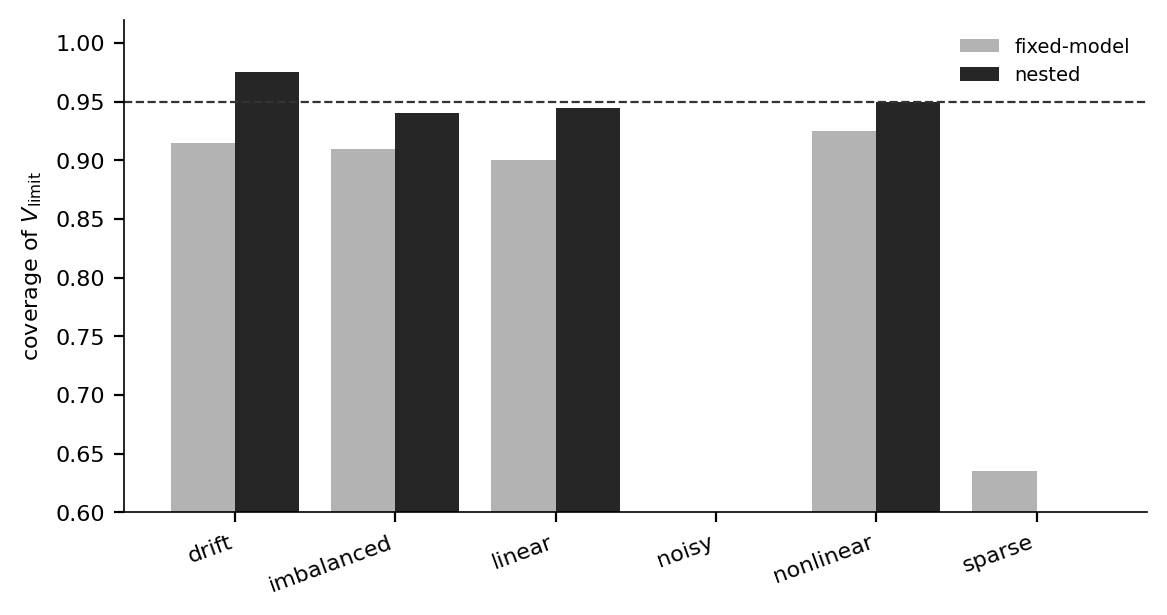
\includegraphics[width=0.9\linewidth]{figS6_coverage.png}
\caption{Coverage of the estimator's own limit in \nWorlds\ simulated worlds,
by interval construction, with Monte Carlo error bars. The dashed line is
nominal. The fixed-model percentile interval is the conventional one; the
nested basic interval is the one this paper reports. The sparse world is where
they disagree by more than a few points, and the nested percentile bar there
is the failure the basic construction repairs.}
\label{fig:coverage}
\end{figure}

\begin{table}[t]
\centering
\small
\resizebox{\ifdim\width>\linewidth\linewidth\else\width\fi}{!}{%%
\begin{tabular}{lrrrrrrrrr}
\toprule
world & bias vs limit & width (basic) & fixed pct & fixed basic & fixed bc & nested pct & nested basic & nested bc & m-out-of-n \\
\midrule
drift & 0.000 & 0.037 & 0.919 & 0.917 & 0.914 & 0.966 & 0.919 & 0.920 & -- \\
imbalanced & $-$0.010 & 0.116 & 0.906 & 0.906 & 0.900 & 0.933 & 0.933 & 0.923 & -- \\
linear & $-$0.002 & 0.060 & 0.925 & 0.931 & 0.915 & 0.939 & 0.931 & 0.921 & 0.768 \\
noisy & $-$0.002 & 0.036 & 0.926 & 0.924 & 0.916 & 0.936 & 0.948 & 0.939 & -- \\
nonlinear & $-$0.002 & 0.044 & 0.923 & 0.923 & 0.924 & 0.940 & 0.929 & 0.929 & 0.758 \\
sparse & $-$0.012 & 0.034 & 0.631 & 0.643 & 0.620 & 0.372 & 0.899 & 0.631 & 0.728 \\
\bottomrule
\end{tabular}%
}
\caption{Coverage of the estimator's own limit $V_{\mathrm{limit}}$ in each simulated world, under seven interval constructions, at the replicate count of Section~\ref{sec:sim}, with the estimator's bias against that limit and the mean width of the interval this paper reports. Nominal is $0.95$; the Monte Carlo standard error on a coverage is \simCoverageSE\ percentage points, so differences below about a point are not differences. An empty cell is a construction not priced on that world.}
\label{tab:sim31}
\end{table}


\begin{table}[t]
\centering
\small
\resizebox{\ifdim\width>\linewidth\linewidth\else\width\fi}{!}{%%
\begin{tabular}{llrrrrlr}
\toprule
n train & K & basic coverage & pct coverage & basic mean width & pct mean width & replicates & coverage se (pp) \\
\midrule
2000 & 20 & 0.887 & 0.887 & 0.085 & 0.085 & 150 & 2.588 \\
2000 & 200 & 0.780 & 0.480 & 0.042 & 0.042 & 150 & 3.382 \\
2000 & 1000 & 0.453 & 0.100 & 0.064 & 0.064 & 150 & 4.065 \\
4000 & 20 & 0.900 & 0.907 & 0.057 & 0.057 & 150 & 2.449 \\
4000 & 200 & 0.907 & 0.500 & 0.031 & 0.031 & 150 & 2.375 \\
4000 & 1000 & 0.507 & 0.080 & 0.047 & 0.047 & 150 & 4.082 \\
8000 & 20 & 0.893 & 0.900 & 0.039 & 0.039 & 150 & 2.520 \\
8000 & 200 & 0.893 & 0.480 & 0.021 & 0.021 & 150 & 2.520 \\
8000 & 1000 & 0.613 & 0.033 & 0.034 & 0.034 & 150 & 3.976 \\
8000 & 3019 & 0.213 & 0.000 & 0.026 & 0.026 & 150 & 3.345 \\
\bottomrule
\end{tabular}%
}
\caption{Sample size and register cardinality varied jointly. Coverage of $V_{\mathrm{limit}}$ and mean interval width for the nested percentile and the nested basic construction. The last row is the cardinality regime of the case study's own register. \emph{How well these are determined.} Every cell is \simGridReps\ replicates, not the \simCoreReps\ of the core experiment, and the coverages here are far from nominal --- so the Monte Carlo standard error of a coverage in this table has a median of \simGridSEMedian\ percentage points and reaches \simGridSEMax, against the \simCoverageSE\ that Section~\ref{sec:simsensitivity} quotes for the core. It is \simGridSERatio\ times larger, it is computed at each cell's own observed rate rather than at the nominal one, and it is a column here rather than a sentence because the differences down this table are read row against row.}
\label{tab:sim31grid}
\end{table}


\begin{table}[t]
\centering
\small
\resizebox{\ifdim\width>\linewidth\linewidth\else\width\fi}{!}{%%
\begin{tabular}{lrrr}
\toprule
world & block multiplier & nested basic & nested pct \\
\midrule
linear & 0.500 & 0.896 & 0.944 \\
linear & 1.000 & 0.920 & 0.908 \\
linear & 2.000 & 0.916 & 0.932 \\
sparse & 0.500 & 0.856 & 0.392 \\
sparse & 1.000 & 0.836 & 0.332 \\
sparse & 2.000 & 0.872 & 0.408 \\
\bottomrule
\end{tabular}%
}
\caption{Three block lengths around $n^{1/3}$: the multiplier column is the factor applied to the rule of thumb, so $0.5$ halves the block and $2$ doubles it. Coverage of $V_{\mathrm{limit}}$.}
\label{tab:sim31block}
\end{table}


\begin{table}[t]
\centering
\small
\resizebox{\ifdim\width>\linewidth\linewidth\else\width\fi}{!}{%%
\begin{tabular}{llllrrrrrr}
\toprule
family & draws are & K & draws & multiplier & mult., MC upper & empirical & emp., OS upper & Rademacher & per-cell \\
\midrule
decision-curve & degenerate & 248 & 200 & 0.803 & 0.805 & 0.935 & 0.964 & 0.785 & 0.937 \\
decision-curve & degenerate & 1100 & 400 & 0.929 & 0.930 & 0.948 & 0.962 & 0.773 & 0.940 \\
decision-curve & gaussian & 248 & 200 & 0.932 & 0.933 & 0.918 & 0.959 & 0.921 & 0.941 \\
decision-curve & gaussian & 1100 & 400 & 0.932 & 0.936 & 0.920 & 0.954 & 0.925 & 0.945 \\
decision-curve & heavy & 248 & 200 & 0.912 & 0.914 & 0.936 & 0.961 & 0.900 & 0.940 \\
decision-curve & heavy & 1100 & 400 & 0.913 & 0.915 & 0.938 & 0.955 & 0.904 & 0.944 \\
decision-curve & nonzero & 248 & 200 & 0.903 & 0.906 & 0.932 & 0.964 & 0.889 & 0.940 \\
decision-curve & nonzero & 1100 & 400 & 0.921 & 0.921 & 0.943 & 0.957 & 0.915 & 0.946 \\
whole-surface & degenerate & 180 & 400 & 0.923 & 0.924 & 0.945 & 0.966 & 0.920 & 0.946 \\
whole-surface & gaussian & 180 & 400 & 0.943 & 0.945 & 0.936 & 0.959 & 0.936 & 0.946 \\
whole-surface & heavy & 180 & 400 & 0.915 & 0.919 & 0.947 & 0.967 & 0.913 & 0.945 \\
whole-surface & nonzero & 180 & 400 & 0.925 & 0.927 & 0.946 & 0.971 & 0.920 & 0.946 \\
\bottomrule
\end{tabular}%
}
\caption{Family-wise coverage of the max-$t$ band against a known answer, over synthetic families matched to this corpus in size, cross-cell correlation and per-cell excess kurtosis, and spanning draw counts around the one it runs. EVERY ROW IS A FAMILY THE CORPUS RUNS: \textsf{whole-surface} at $K = \nCellsPerPairMedian$ and \nDrawsSurface\ draws is every pair's surface family, \textsf{decision-curve} at $K = \nDcaFamilyModal$ and \nDrawsSurface\ draws the modal curve family, and the \nDcaFamily-cell row at \nDcaDraws\ draws the case study's own curve family; the draw-count ladder the text quotes is a sensitivity around the first and is not printed here. Nominal is $0.95$; the five middle columns are the five candidate critical values and the last is the control. \emph{The bootstrap here is ideal} --- the draws come from the sampling distribution itself --- so every coverage in this table is an upper bound on what the real procedure attains, and the control says why: \emph{per-cell} is the basic interval the band is built from, on the same draws, and it is short of nominal before any multiplicity correction is applied. \emph{Regimes.} \textsf{gaussian} is the case the multiplier bootstrap is derived for; \textsf{heavy} carries this corpus's measured tails; \textsf{degenerate} adds the cells whose net-benefit difference is zero by arithmetic, which the corpus's decision-curve families contain and its surface families do not; \textsf{nonzero} is heavy with a fixed heterogeneous non-zero truth, the regime under which a cell can be resolved correctly and a region label is actually being asked to hold. Every cell is \nBandCoverageReps\ replicates, so no coverage here is determined worse than \bandCoverageSEMax.}
\label{tab:bandcov}
\end{table}


\begin{table}[t]
\centering
\small
\resizebox{\ifdim\width>\linewidth\linewidth\else\width\fi}{!}{%%
\begin{tabular}{lllrlrrrrrrr}
\toprule
world & n train & K & K / n & replicates & coverage at c = 1 & se & c & c lo & c hi & c applied & c log-linear \\
\midrule
linear & 180000 & 200 & 0.001 & 500 & 0.882 & 0.014 & 1.352 & 1.174 & 1.482 & 1.177 & 1.000 \\
linear & 8000 & 20 & 0.003 & 500 & 0.916 & 0.012 & 1.154 & 1.073 & 1.307 & 1.177 & 1.000 \\
linear & 4000 & 20 & 0.005 & 500 & 0.898 & 0.014 & 1.219 & 1.101 & 1.313 & 1.177 & 1.056 \\
linear & 2000 & 20 & 0.010 & 500 & 0.924 & 0.012 & 1.108 & 1.024 & 1.228 & 1.177 & 1.134 \\
linear & 50000 & 625 & 0.013 & 498 & 0.902 & 0.013 & 1.296 & 1.135 & 1.689 & 1.177 & 1.160 \\
linear & 8000 & 100 & 0.013 & 500 & 0.936 & 0.011 & 1.096 & 0.960 & 1.203 & 1.177 & 1.160 \\
sparse & 8000 & 100 & 0.013 & 500 & 0.892 & 0.014 & 1.317 & 1.220 & 1.453 & 1.177 & 1.160 \\
linear & 2000 & 25 & 0.013 & 500 & 0.908 & 0.013 & 1.188 & 1.072 & 1.277 & 1.177 & 1.160 \\
linear & 750 & 10 & 0.013 & 500 & 0.920 & 0.012 & 1.117 & 1.029 & 1.207 & 1.177 & 1.168 \\
linear & 4000 & 100 & 0.025 & 500 & 0.896 & 0.014 & 1.179 & 1.087 & 1.296 & 1.177 & 1.245 \\
linear & 8000 & 200 & 0.025 & 499 & 0.932 & 0.011 & 1.093 & 0.985 & 1.264 & 1.177 & 1.245 \\
sparse & 4000 & 200 & 0.050 & 500 & 0.884 & 0.014 & 1.182 & 1.131 & 1.299 & 1.177 & 1.337 \\
linear & 2000 & 100 & 0.050 & 500 & 0.912 & 0.013 & 1.234 & 1.055 & 1.326 & 1.177 & 1.337 \\
linear & 4000 & 200 & 0.050 & 500 & 0.888 & 0.014 & 1.195 & 1.119 & 1.337 & 1.177 & 1.337 \\
linear & 8000 & 400 & 0.050 & 500 & 0.884 & 0.014 & 1.152 & 1.104 & 1.226 & 1.177 & 1.337 \\
linear & 750 & 38 & 0.051 & 500 & 0.926 & 0.012 & 1.103 & 0.989 & 1.259 & 1.177 & 1.338 \\
sparse & 2000 & 200 & 0.100 & 500 & 0.836 & 0.017 & 1.333 & 1.224 & 1.372 & 1.310 & 1.435 \\
linear & 500 & 50 & 0.100 & 500 & 0.874 & 0.015 & 1.250 & 1.141 & 1.460 & 1.310 & 1.435 \\
linear & 4000 & 400 & 0.100 & 499 & 0.796 & 0.018 & 1.287 & 1.221 & 1.399 & 1.310 & 1.435 \\
linear & 2000 & 200 & 0.100 & 500 & 0.844 & 0.016 & 1.316 & 1.253 & 1.417 & 1.310 & 1.435 \\
linear & 8000 & 1000 & 0.125 & 496 & 0.655 & 0.021 & 1.526 & 1.417 & 1.600 & 1.441 & 1.468 \\
linear & 2000 & 250 & 0.125 & 500 & 0.792 & 0.018 & 1.404 & 1.284 & 1.485 & 1.441 & 1.468 \\
linear & 750 & 94 & 0.125 & 500 & 0.872 & 0.015 & 1.310 & 1.154 & 1.396 & 1.441 & 1.468 \\
linear & 2000 & 400 & 0.200 & 500 & 0.758 & 0.019 & 1.562 & 1.398 & 1.670 & 1.562 & 1.540 \\
sparse & 4000 & 1000 & 0.250 & 498 & 0.460 & 0.022 & 1.716 & 1.672 & 1.849 & 1.727 & 1.575 \\
linear & 4000 & 1000 & 0.250 & 500 & 0.520 & 0.022 & 1.739 & 1.632 & 1.805 & 1.727 & 1.575 \\
linear & 8000 & 3019 & 0.377 & 488 & 0.305 & 0.021 & 1.881 & 1.804 & 1.988 & 1.791 & 1.643 \\
linear & 500 & 200 & 0.400 & 500 & 0.760 & 0.019 & 1.450 & 1.353 & 1.656 & 1.791 & 1.653 \\
linear & 2000 & 1000 & 0.500 & 500 & 0.462 & 0.022 & 1.869 & 1.788 & 2.024 & 1.869 & 1.691 \\
\bottomrule
\end{tabular}%
}
\caption{The coverage calibration. For each cell of the $(n, K)$ plane: the coverage the reported interval actually attains, and the factor $c$ by which it must be widened to attain the nominal level, with the Monte Carlo interval of that factor. $c$ is the $0.95$ quantile of the studentised error and is computed, not searched for. `c applied' is the monotone regression the corpus is calibrated with; `c log-linear' is the parametric fit whose slope Section~\ref{sec:regions} quotes, printed beside it because it sits below the measured factor at small ratios and would under-correct there.}
\label{tab:plane}
\end{table}



%%  ROUND TWENTY-SEVEN.  Both documents promised these two and neither
%%  compiled them.  The article's front matter (Section 1) and this
%%  supplement's own abstract each list "the correction register" among the
%%  supplement's contents, and the archive description cites it by name --
%%  while `app_corrections' and `app_pilot' were reachable only from
%%  `_appendix_block.tex', which no built document includes.  A promise a
%%  referee can check in one click is worth more attention than a page count.
\section{A reporting standard, and software}
\label{app:standard}
\input{parts/app_standard}

\section{The correction register}
\label{app:corrections}

This project keeps a correction register. Earlier versions of this work
carried it in the main text; a referee for this journal observed that
scientific transparency should be visible in the design and the supplement
rather than repeatedly asserted, and that is right, so it is here.

\texttt{REFEREE-LOG.md} in the archive carries every objection this project
has received, each with its disposition and with the corrections it produced
named. What follows is the register grouped by \emph{class}, because the
classes are more useful than the incidents: they say what kind of mistake this
apparatus is prone to. Identifiers run in the order the corrections were made,
across all twenty rounds; three of the low numbers never entered the register
and the classes below are therefore not a contiguous range, which is a fact
about the numbering and not a missing entry.

\paragraph{Class A --- a control that could not fail}
Four corrections (C1, C2, C8, C16) are nulls or searches drawn at the wrong
level, swept over the wrong range, or given fresh noise inside a comparison
that assumed determinism. A null that cannot fail is worse than no null,
because it is reported as evidence. The most recent, C16, is in
\ref{app:props}: the axis non-redundancy search drew fresh noise
inside each cell evaluation, so two evaluations of the same cell disagreed and
the search found almost nothing.

\paragraph{Class B --- a quantity whose sign was set by a tie-break}
Two corrections (C4, C7) concern an operational factor computed at a fixed
review capacity, where $93.1\%$ of what the naive baseline nominated came from
a single tied block and reordering rows inside that block moved the arm from
$-26$ to $+608$. A quantity whose sign is set by a tie-break is not a
measurement. Section~\ref{sec:dca} is built on net benefit, which admits or
excludes a whole tied block at a threshold and never breaks one.

\paragraph{Class C --- every literal correct, the relation between them
false}
Five corrections (C9, C10, C12, C13, C14) are sentences in which each printed
number was right and the claim asserted about them was not: an extremum that
was the worst of the points the table happened to name; a count reported as a
contiguous run; a range ``across the operating range'' that was a range across
five named points; a universal ``if and only if'' whose necessity direction is
only existential (Section~\ref{sec:props}); and --- the one that mattered most
--- a headline spread that was inflated by an intercept-only baseline no
analyst would build, while a later section of the same manuscript said so and
the abstract did not. This class is the reason
Section~\ref{sec:regionsdef} excludes the intercept-only rung by definition and
the reason every number in this document is a generated macro rather than a
typed literal.

\paragraph{Class D --- evidence one download away}
One correction (C11): an earlier version reported that it could not establish
whether the knowledge-article reference was available at incident creation,
named the file that would settle where the field comes from, and did not
obtain it. Obtaining it changed the headline. Section~\ref{sec:cmdb} now
reports two decision times rather than choosing one, because obtaining the
file settled where the field is written and not when.

\paragraph{Class E --- a claim about the world that our own coder could not
support}
One correction (C15), and it is the largest. An earlier version reported that
\emph{not one} of twenty audited papers reports the increment across a range
of operating points. The rebuilt pilot of Section~\ref{sec:practice}
adjudicates the papers the mechanical screen \emph{rejected} as well as the
ones it accepted, measures the screen's sensitivity at \auditSens, and finds
eligible papers that do report the increment across a range of operating
points --- one of them at four values of $k$ in a top-$k$ evaluation. The
earlier ``not one'' was a property of a coder that finds fewer than half of
the eligible papers, not a property of the literature. The corrected estimate
is \auditRangeThresholdPct\ with an interval that includes it.

\paragraph{Class F --- internal inconsistency}
Four corrections (C17, C18, C19, C22) are places where an earlier manuscript
disagreed with itself: an instrument count that treated two thresholds of one
instrument as two instruments; a reference reduction quoted as
$43.7\%$ in the text and $35.0\%$ in a table without the change of
specification being made clear; and a section that said a withdrawn
instrument was retained in a table that did not contain it. The generated-macro
discipline of \ref{app:verifier} makes this class structurally
impossible rather than merely unlikely --- and does not make it impossible
when the same wrong quantity is computed twice from the same wrong expression,
which is C22. Correcting the pilot's frame size in the facts and not in the
PRISMA flow left Section~\ref{sec:practice} reading
\nAuditFrame\ and Table~\ref{tab:prisma} reading two orders of magnitude more, four pages apart,
\emph{after} the error had been found and written up. The frame is computed
once now, before both consumers, and the verifier checks every row of the flow
that the prose also quotes.

\paragraph{Class G --- an estimand that was not the one being estimated}
One correction (C20), found in round nineteen and the reason
\ref{app:noisy} exists. The simulation of Section~\ref{sec:sim}
computed both estimands by enumerating the data generator's cells, which in
the noisy world carry the register's \emph{true} value while the estimator
only ever observes a value replaced by a uniform draw with probability
\simNoiseRate. Coverage was therefore measured against a population the
estimator does not sample from, and came out at \coverageNoisyBefore\ with an
apparent bias of \biasNoisyBefore. Both were artefacts. The correction is
exact marginalisation of the noise; the estimator's mean was
\meanNoisyEstimate\ before and after.

This class is worth separating from Class F because nothing in the
generated-macro discipline could have caught it: every number was internally
consistent, correctly computed, and correctly printed. What was wrong was the
\emph{definition} of the quantity two of them referred to. It was found by
constructing two experiments that could each have confirmed the comfortable
reading --- that the method simply fails in that world --- and having both
refuse to. That is the only mechanism in this project that has ever caught an
error of this class, and it is not automatable.

\paragraph{Class H --- a statistic aggregated over the wrong index set}
One correction (C21). The practice pilot's frame size summed a stratum-size
column over the \emph{rows} of the sample rather than over its distinct
strata, and a stratum's size is carried on every row of that stratum. The
quantity computed was $\sum_h N_h n_h$ and the quantity intended was
$\sum_h N_h$, so a frame of \nAuditFrame\ records was reported as one two
orders of magnitude larger. Every input was correct; the arithmetic was
correct; the group-by was wrong.

The correction changed what the pilot \emph{is} and not only how large it
sounds. With the true frame in view it is immediate that the design weight is
\auditMaxWeight\ in every stratum, that the enumeration stopped short of its
declared budget of \nAuditTarget, and that the pilot is therefore a census of
what one index returned rather than a probability sample of a literature ---
which Section~\ref{sec:practice} now says, with the additional limit that the
frame's coverage of the field is unmeasured.

The guard is a re-derivation rather than a recount: the verifier computes the
frame from the sample by grouping, and refuses a manuscript in which a frame
is smaller than the sample it contains, or differs from it while every design
weight is one. A checker that recomputed the same aggregation would have
agreed with the error.

\paragraph{Class I --- an inferential object whose denominator was not the
one the claim quantified over}
Two corrections (C26, C28), and they are the same mistake in two places. A
region label such as \emph{uniformly beneficial} ranges over every admissible
cell of a surface, and an earlier version supported it with max-$t$ bands
whose family was the five scalar instruments \emph{at one cell}; the family
was two orders of magnitude smaller than the claim. Widening it to the whole
surface raises the critical value from \maxTWithinMedian\ to
\maxTSurfaceMedian\ at the median pair and changes the region label on
\nRegionChangedByFamily\ of \nPairs\ pairs --- and more at the cell level,
where a region label's coarseness no longer hides it and the wider family
unresolves cells throughout. Section~\ref{sec:simbands} now
declares four interval objects by name so a table cannot print one and be read
as the other. The same class covers the
pilot's Wilson intervals (C28): a binomial interval was put around a ratio of
two weighted totals through a fractional ``effective sample size'', and none
of the five resulting intervals contains its design-based counterpart.

The general form is worth stating because it is not a coding error and no
checker in this repository would have caught it: \textbf{an interval is only
as good as the correspondence between the family it controls and the sentence
it is used to license}, and that correspondence is a judgement about English,
not a property of the arithmetic.

\paragraph{Class J --- a quantity assembled from units that do not add}
Two corrections (C25, C27). The first: an earlier version reported the largest
per-axis difference $\max_i(S_{T_i} - S_i)$ and described it as the share of
variance carried by interactions. Those differences overlap across axes ---
a two-way component appears in the total effect of both of its axes --- so
their maximum is neither their sum nor their union, and the total higher-order
share is $1 - \sum_i S_i$, which on this corpus is \interactionTotalPct\
against the \largestInvolvementPct\ that was printed. The second: expected
regret was averaged over an admissible set spanning five scalar instruments
and reported as a single percentage ``in the metric's own units''. There is no
such unit once AUC and Brier skill are inside one average.
Section~\ref{sec:rules} now reports regret inside one instrument at a time,
and Section~\ref{sec:nbregret} reports a common-utility version on calibrated
net benefit, which is a scale on which averaging is defined.

\paragraph{Class K --- a theorem stated wider than its proof, and wider than
the truth}
Two corrections (C23, C24). The necessity direction of the rank-invariance
proposition quantified over every non-rank-based instrument and was supported
by one stored configuration for five named instruments under one map. Repairing
the proof also refuted the claim: what invariance of the \emph{reduction}
requires is that the recalibration act \emph{affinely} on the instrument, not
that it leave it fixed, and Section~\ref{sec:props} exhibits a
non-rank-based instrument whose reduction is invariant. The word
\emph{exactly} was wrong, not merely unproved. C24 withdraws the axis
non-redundancy search entirely: its answer moved with an arbitrary tolerance,
no claim depended on it, and removing it was cheaper than repairing it.

\paragraph{Class L --- a number the design cannot produce, and a word the
design does not license}
Two corrections (C29, C30). An earlier version printed raw and Holm-adjusted
bootstrap $p$-values of $0.000$ from 200 draws; no finite bootstrap can
produce zero,
and Section~\ref{sec:planned} now uses the plus-one estimator with the
smallest attainable value stated beside it. And the five contrasts were called
\emph{confirmatory} when they had been fixed after eighteen rounds of analysis
on the same data; they are \emph{final-round planned contrasts}, which is
what the design supports.

\paragraph{Class M --- an interpretation attached to a scale that does not
carry it}
One correction (C31). Decision-curve thresholds were read as probability
thresholds,
and therefore as cost ratios, on scores whose calibration slope was reported
in the same manuscript as far from one. Section~\ref{sec:calibfirst} refits
every model contributing to a decision-curve conclusion under a training-only
calibration and labels raw-score curves as score-threshold sensitivity
analyses, which is what they are.

\paragraph{What found these, and what to take from it}
Of the corrections above, those found in the project's own work divide by
\emph{method} rather than by class. The estimand error (C20) was found by
constructing two experiments that could each have confirmed the comfortable
reading and having both refuse. The aggregation error (C21) and the
inconsistency it left behind (C22) were found by reading the compiled pages.
So were five defects that produced no wrong number at all but printed badly:
the word \emph{Appendix} doubled on every appendix reference, a macro eating
the space before an em dash, a macro carrying words set as italic variables, a
sentence's tail printed twice, and a minus sign set as a hyphen in the
sentence about signs.

Every checker in this repository ran clean on the build that carried all of
them. That is the finding worth generalising: an apparatus that guarantees
every number is derived from a result file guarantees nothing about whether
the sentence around it says what the author meant, and the only instrument
that has ever caught that is somebody reading the output.


\section{The literature pilot in full}
\label{app:pilot}

Section~\ref{sec:practice} states what the pilot is and what it is not. This
appendix gives the flow, the design and the numbers.

\subsection*{Flow}

\begin{table}[t]
\centering
\small
\resizebox{\ifdim\width>\linewidth\linewidth\else\width\fi}{!}{%%
\begin{tabular}{lr}
\toprule
step & n \\
\midrule
records enumerated in the frame & 54910.000 \\
records sampled & 600.000 \\
full text retrieved & 369.000 \\
full text not retrieved & 231.000 \\
screened in by the mechanical rule & 54.000 \\
screened out: no quantitative metric & 192.000 \\
screened out: no incremental comparison & 123.000 \\
adjudicated, screened-in stratum (census) & 54.000 \\
adjudicated, screened-out stratum (sample) & 120.000 \\
confirmed eligible, screened-in stratum & 26.000 \\
confirmed eligible, screened-out stratum (unweighted) & 11.000 \\
estimated eligible among all retrieved full texts & 54.900 \\
\bottomrule
\end{tabular}%
}
\caption{The pilot's flow, in PRISMA-style steps.}
\label{tab:prisma}
\end{table}


Table~\ref{tab:prisma} is the flow, laid out in the style
\citet{page2021prisma} prescribe for a systematic review --- which this is
not, and the appendix says so throughout; the layout is used because it makes
what was excluded, and why, countable. Records were enumerated from
a public index across \nAuditStrata\ strata --- venues, two citation seeds and
a topic frame --- and the enumeration is cached per stratum in the archive so
it can be re-run without re-querying.

The allocation was declared before the enumeration finished: proportional to
stratum size with a floor of \minPerStratum\ per stratum, up to a budget of
\nAuditTarget\ records, with every estimate carrying the design weight
$N_h / n_h$. The enumeration returned \nAuditFrame\ deduplicated records ---
short of that budget, because the provider's daily request quota was exhausted
first --- so the allocation bound at $n_h = N_h$ in every stratum and the
design weight is \auditMaxWeight\ throughout. \textbf{The machinery of
weighting is therefore inert here.} It is retained because it is what makes
the design re-runnable at scale, and because a reader is entitled to see that
the weights are one rather than to assume it; but the pilot's reach is that of
a census of \nAuditFrame\ enumerated records, not that of a probability sample
of a literature, and Section~\ref{sec:practice} says so.

\subsection*{The two-stratum adjudication, and why it is the point}

\begin{table}[t]
\centering
\small
\resizebox{\ifdim\width>\linewidth\linewidth\else\width\fi}{!}{%%
\begin{tabular}{lrrrl}
\toprule
quantity & estimate & lo & hi & note \\
\midrule
screen sensitivity & 0.474 & 0.347 & 0.602 & weighted; the screened-out stratum is a 38.1\% sample \\
screen specificity & 0.911 & 0.874 & 0.938 & weighted \\
screen precision (PPV) & 0.481 & 0.354 & 0.611 & census over the screened-in stratum \\
eligibility prevalence among retrieved full texts & 0.149 & -- & -- & two-stratum estimate \\
\bottomrule
\end{tabular}%
}
\caption{The mechanical screen's measured accuracy against the adjudicated standard.}
\label{tab:screenacc}
\end{table}


The design's one non-obvious feature is that the papers the mechanical screen
\emph{rejected} were sampled and adjudicated too. Without that, a screen's
misses are invisible and its proportions can only be described as bounds ---
which an earlier version of this work did, incorrectly, because a screen with
false positives does not yield a bound in either direction.

With it, Table~\ref{tab:screenacc} reports what the screen actually does:
sensitivity \auditSens\ [\auditSensLo, \auditSensHi], specificity
\auditSpec, precision \auditPrec. Agreement between the mechanical codes and
the adjudicated ones has median $\kappa = \auditKappa$, which is poor. The
prevalence estimates in Table~\ref{tab:pilot} are nonetheless unbiased for the
adjudicated standard, because the two strata are combined with their sampling
weights rather than the screened-in stratum being used alone. That is why no
sensitivity-and-specificity correction of the \citet{rogan1978estimating} kind
is applied: such a correction repairs a prevalence estimated \emph{from the
screen}, and the estimate here is made from the adjudications, with the screen
entering only as the stratifier.

\subsection*{Two mechanical screens, one standard}

\begin{table}[t]
\centering
\small
\resizebox{\ifdim\width>\linewidth\linewidth\else\width\fi}{!}{%%
\begin{tabular}{lrrrr}
\toprule
rule & sensitivity & specificity & precision & n flagged \\
\midrule
amended (primary) & 0.474 & 0.911 & 0.481 & 54 \\
registered & 0.569 & 0.769 & 0.301 & 73 \\
\bottomrule
\end{tabular}%
}
\caption{Two mechanical screens against the same adjudicated standard. They fail differently and neither is good enough to support a claim about a field's practice, which is why the pilot does not make one.}
\label{tab:twoscreens}
\end{table}


Two screening rules ran on every paper: the one registered in
\texttt{AUDIT-PROTOCOL.md} section~4, and the amended one of its
amendment~1, written against the same prose. Table~\ref{tab:twoscreens}
reports both against the adjudicated standard. They fail differently --- the
registered rule flags more papers and is right about fewer of them --- and
neither is good enough to support a claim about a field's practice. That is
the pilot's central finding about itself.

\subsection*{Applicability-specific denominators}

\begin{table}[t]
\centering
\small
\resizebox{\ifdim\width>\linewidth\linewidth\else\width\fi}{!}{%%
\begin{tabular}{lr}
\toprule
quantity & n \\
\midrule
eligible papers & 54.875 \\
of which the incremental feature is a lookup into an external register or reference source & 3.000 \\
of those, reporting the increment across a range of register populations & 0.000 \\
\bottomrule
\end{tabular}%
}
\caption{Applicability-specific denominators.}
\label{tab:applicability}
\end{table}


Not every code applies to every eligible paper. The register-population code
is meaningful only where the incremental feature is a lookup into an external
register or reference source whose per-case coverage can be incomplete, and
Table~\ref{tab:applicability} reports that denominator separately. Of
\nAuditEligible\ estimated eligible papers, \nAuditApplicable\ have such a
feature. A proportion of zero over a denominator of \nAuditApplicable\ is a
much weaker statement than a proportion of zero over \nAuditEligible, and the
earlier version reported the latter.

\subsection*{What is missing, and what it could do}

\begin{table}[t]
\centering
\small
\begin{tabular}{lrr}
\toprule
characteristic & retrieved & not\_retrieved \\
\midrule
n & 369.000 & 231.000 \\
median year & 2023.000 & 2024.000 \\
share from the four round-eighteen venues & 0.650 & 0.654 \\
\bottomrule
\end{tabular}

\caption{Retrieved against unretrieved records, and the bounds on the eligibility rate under the extreme assumptions about the unretrieved.}
\label{tab:missing}
\begin{tabular}{lr}
\toprule
assumption & p\_eligible \\
\midrule
none of the unretrieved papers is eligible & 0.091 \\
the unretrieved papers are eligible at the retrieved rate & 0.149 \\
all of the unretrieved papers are eligible & 0.476 \\
\bottomrule
\end{tabular}
\end{table}


Full text was unavailable for \nAuditNoFullText\ of the sampled records.
Table~\ref{tab:missing} compares the retrieved and the unretrieved on every
characteristic the metadata carries, and gives the eligibility rate under the
extreme assumptions that none and that all of the unretrieved are eligible:
\auditBoundLo\ to \auditBoundHi. The retrieved and unretrieved sets do not
differ materially on year or venue mix, which is reassuring and is not
evidence of exchangeability.

\subsection*{What this design can and cannot resolve}

\begin{table}[t]
\centering
\small
\resizebox{\ifdim\width>\linewidth\linewidth\else\width\fi}{!}{%%
\begin{tabular}{rll}
\toprule
half width & n required & achieved \\
\midrule
0.050 & 385 & 29.6 \\
0.070 & 196 & 29.6 \\
0.100 & 97 & 29.6 \\
0.150 & 43 & 29.6 \\
0.200 & 25 & 29.6 \\
\bottomrule
\end{tabular}%
}
\caption{What the pilot's design can and cannot resolve: the adjudicated sample each half-width would need, against the effective sample the pilot achieved.}
\label{tab:power}
\end{table}


An effective sample of \nAuditEffective\ resolves a proportion near one half
to about $\pm\auditHalfWidthPct$ percentage points. A design that resolved it
to $\pm 7$ would need \nAuditRequired\ adjudicated eligible papers.
Table~\ref{tab:power} gives the requirement at five half-widths. This is the
single most important limitation of the pilot and it is why no claim in the
paper depends on it.

\subsection*{Adjudication materials}

Every adjudication was made from an evidence dossier extracted from the paper's
full text: the sentences the screen fired on, the sentences carrying a
performance metric beside a number, and the neighbourhood of every mention of
each coded concept. The dossiers are committed to
\texttt{data/audit2/dossiers/} and the judgements to
\texttt{data/audit2/adjudication\_in.csv} and
\texttt{adjudication\_out.csv}, with a free-text reason for every one. There
is one adjudicator, machine-assisted; that is transparency, not independence,
and Section~\ref{sec:practice} says so.

\subsection*{The prevalence estimates, and their denominators}

\begin{table}[t]
\centering
\small
\resizebox{\ifdim\width>\linewidth\linewidth\else\width\fi}{!}{%%
\begin{tabular}{lrrrrrrr}
\toprule
code & estimate & boot lo & boot hi & design lo & design hi & Wilson lo & Wilson hi \\
\midrule
B\_stated & 0.850 & 0.705 & 0.973 & 0.755 & 0.945 & 0.682 & 0.937 \\
B\_justified & 0.175 & 0.067 & 0.315 & 0.102 & 0.249 & 0.078 & 0.347 \\
M\_justified & 0.055 & 0.000 & 0.129 & 0.042 & 0.067 & 0.013 & 0.198 \\
Theta\_stated & 0.271 & 0.121 & 0.442 & 0.162 & 0.380 & 0.144 & 0.450 \\
Range\_reported & 0.440 & 0.264 & 0.619 & 0.317 & 0.562 & 0.278 & 0.615 \\
\bottomrule
\end{tabular}%
}
\caption{The pilot's proportions over the estimated eligible population, with the stratified bootstrap interval this paper reports, the design-based linearised interval beside it, and the Wilson interval an earlier version printed. None of the five Wilson intervals is contained in its design-based counterpart.}
\label{tab:pilot}
\end{table}


Over an estimated \nAuditEligible\ eligible papers with an effective sample
size of \nAuditEffective: \auditBStatedPct\ state the composition of their
baseline; \auditBJustifiedPct\ argue for what the baseline excludes;
\auditMJustifiedPct\ argue for the metric; \auditThetaStatedPct\ state or
integrate over an operating point; \auditRangeBaselinePct\ report the
increment at more than one baseline, \auditRangeMetricPct\ under more than one
metric, \auditRangeThresholdPct\ across a range of operating points and
\auditRangePopulationPct\ across a range of register populations.

Denominators are applicability-specific. Only \nAuditApplicable\ of the
eligible papers have an incremental feature that is a lookup into an external
register at all, so the population axis has a denominator of
\nAuditApplicable\ and not of \nAuditEligible. Using the eligible count for
every axis understates every rate whose axis does not apply to every paper,
and is not done here.

\paragraph{Variance}
Each proportion here is a \emph{ratio} of two weighted totals: the numerator
counts eligible papers carrying a code, the denominator estimates the eligible
population, and both are random. The screened-in stratum is a census, so it
carries a design weight of \auditWeightIn\ and contributes no sampling
variance; the screened-out stratum was adjudicated at a sampling fraction
whose reciprocal is \auditWeightOut.

A \textbf{Wilson} interval computed from a fractional ``effective sample
size'' --- which is what this pilot previously reported --- is a binomial
interval for a binomial count, and neither the numerator nor the denominator
here is one. Table~\ref{tab:pilot} reports instead a
\textbf{stratified nonparametric bootstrap} --- resampling adjudicated papers
within stratum and recomputing the ratio, \nPilotBoot\ times --- as the
primary interval, because with \nAuditOutSampled\ adjudicated papers in the
second stratum a linearisation is not to be trusted, and the
\textbf{design-based} linearised interval beside it. The design-based interval
has a median width of \auditDesignWidthPct\ percentage points and the
bootstrap \auditBootWidthPct, against the Wilson interval's
\auditWilsonWidthPct; and \emph{none} of the five Wilson intervals is
contained in its design-based counterpart, the endpoints differing by up to
\auditMaxGapPct\ percentage points. That is correction~C28 in
\ref{app:corrections}.

\subsection*{Four limits, stated rather than buried}

The frame is what one provider's index returned before its daily quota stopped
the enumeration, so it is a convenience frame and its coverage of the field is
unmeasured; nothing here corrects for that, and nothing can without a second
index.

An effective sample of \nAuditEffective\ resolves a proportion to about
$\pm\auditHalfWidthPct$ percentage points; a design that resolved it to
$\pm 7$ points would need \nAuditRequired\ adjudicated papers. That is the
sample-size calculation, and this pilot does not meet it.

Full text was unavailable for \nAuditNoFullText\ of the sampled records, and
under the extreme assumptions that none or all of them are eligible the
eligibility rate moves between \auditBoundLo\ and \auditBoundHi.

There is one adjudicator, machine-assisted, not two independent human raters.
Every adjudication was made from an evidence dossier committed to the
repository, so the judgements can be re-examined against exactly what they
were made from; that is transparency, not independence, and no inter-rater
reliability statistic reported here is a substitute for a second human.


\bibliographystyle{elsarticle-harv}
\bibliography{references}

\end{document}
